% (c) 2014 Daniele Masini - d.masini.it@gmail.com
\chapter{Equiestensione e aree}

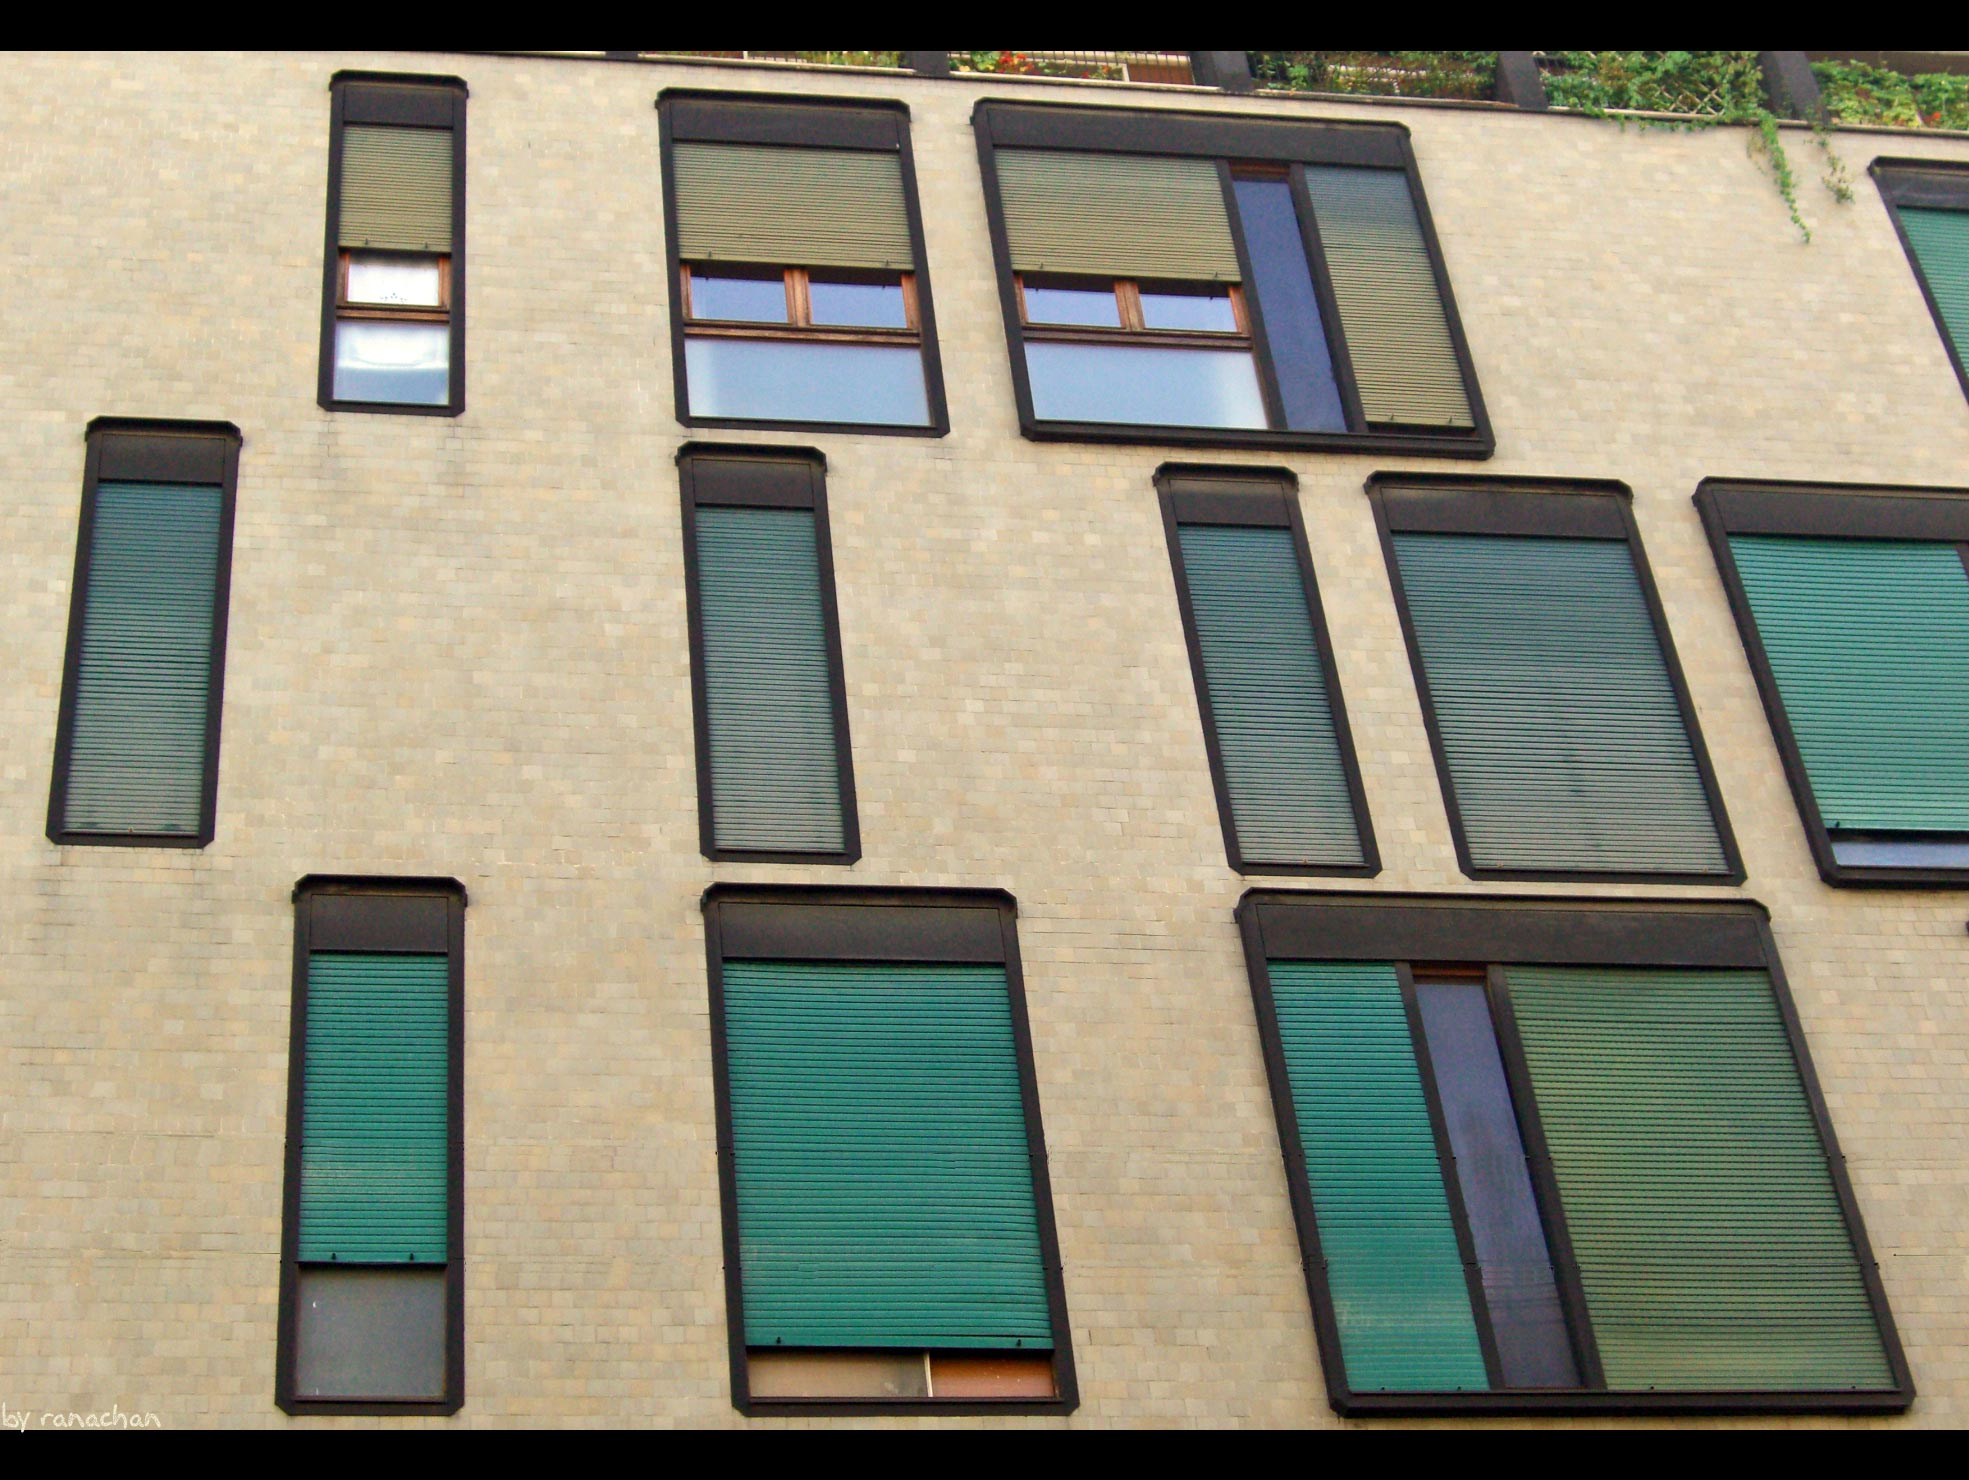
\includegraphics[width=0.95\textwidth]{window_geometry.jpg}
  \begin{center}
    {\large ``Window geometry''}\par
    Foto di midori.no.kerochan\par
    \url{http://www.flickr.com/photos/28661972@N05/2751042868/}\par
    Licenza: Creative Commons Attribution 2.0\par
  \end{center}
\newpage


\section{Estensione superficiale}

Il \emph{tangram}\label{tangram} è un antichissimo gioco cinese. Il nome con cui lo conosciamo si pensa derivato dall'unione della parola \emph{tang} o \emph{tan}, che significa \emph{cinese}, e \emph{gram} che significa \emph{immagine}. Anticamente in Cina era chiamato ``schema intelligente a sette pezzi'' o anche ``le sette pietre della saggezza'' poiché si riteneva che la padronanza del gioco fosse la chiave per ottenere saggezza e talento.
Il gioco è costituito da un quadrato ritagliato in 7 pezzi poligonali aventi in comune solo punti del loro contorno (come mostra la figura ...).

% figura

I pezzi possono essere disposti e accostati gli uni agli altri senza sovrapposizioni in modo da ottenere una grande varietà di figure; la regola base è che devono essere utilizzati tutti i 7 pezzi. Si possono così formare alcuni disegni come mostrato nelle figure ....

Potete osservare che si forma un poligono quando i singoli pezzi vengono accostati mediante un lato: l'uomo seduto è un poligono, ma non la candela; i due poligoni rappresentati sono l'uno concavo e l'altro convesso.

Con tutti i 7 pezzi del gioco si possono costruire 13 poligoni convessi, compreso il quadrato iniziale, provate a costruirli: fotocopiate la pagina precedente e ritagliate i 7 pezzi del tangram.

Evidentemente i 13 poligoni che avrete costruito non sono congruenti, né hanno la stessa forma; potete dire che sono formati dalle stesse parti poligonali, ciascuno può cioè essere pensato come unione dei \emph{tan} aventi in comune almeno un punto del loro perimetro, ma nessun punto interno.


\begin{definizione}
Con \emph{somma} di due \emph{figure piane} $X$ e $Y$, non aventi punti comuni o aventi in comune solo punti del loro contorno, intendiamo la figura $Z$ unione dei punti di $X$ e $Y$ e la indicheremo con $Z=X+Y$. Diremo inoltre che $X$ è la \emph{differenza} tra $Z$ e $Y$ e scriveremo $X=Z-Y$.
\end{definizione}

\begin{definizione}
Due poligoni sono \emph{equicomposti} se sono formati dalle stesse parti poligonali (figure piane).
Due poligoni sono \emph{equiscomponibili} se è possibile decomporre uno di essi in un numero finito di parti poligonali con le quali si possa ricoprire l'altro.
\end{definizione}

Tutte le figure poligonali costruite con i pezzi del tangram sono dunque poligoni equicomposti, ma possono anche essere considerati poligoni equiscomponibili: tale caratteristica si esprime in simboli scrivendo $p_1 \doteq p_2 \doteq \ldots{}$ che si legge ``$p_1$ equicomposto $p_2$ equicomposto \ldots{}''.

Ritagliate da un quadrato i quattro triangoli rettangoli isosceli che si ottengono tracciando le sue diagonali. Disponendo fianco a fianco i triangoli ottenuti in modo che i due lati comuni abbiano la stessa lunghezza, si ottengono 14 figure diverse. Due di esse sono riportate nella figura. Realizzate tutte le altre figure.
Le figure ottenute sono \ldots\ldots\ldots\ldots{} perché sono formate da \ldots\ldots\ldots\ldots{}

(da: Prova di allenamento della gara di ``Matematica senza frontiere'' del 9/02/1994)

Nella figura sono disegnati un quadrato $ABCD$, un rettangolo $PQRS$ avente $PQ=2AB$ e $SP=AB/2$ e un rombo $FGHK$ avente una diagonale uguale al lato del quadrato e l'altra il doppio. Mostrate come sia possibile scomporre ciascuno dei tre poligoni in parti tali da poter ricoprire gli altri due. Puoi concludere che i tre poligoni assegnati sono equiscomponibili? \ldots\ldots{}

Dato l'insieme $F = \{f_1\text{,}f_2\text{,}f_3\}$ delle figure poligonali disegnate a lato, seguite le seguenti istruzioni:\\
\verb|   |\textsl{ripeti:}\\
\verb|      |\textsl{scegli una figura dell'insieme $F$;}\\
\verb|      |\textsl{traccia alcuni segmenti che la decompongano in parti poligonali;}\\
\verb|      |\textsl{forma con le parti ottenute altre 3 figure poligonali;}\\
\verb|   |\textsl{finché non hai esaurito le figure.}\\
Costruite l'insieme $G$ di tutti i poligoni ottenuti con questa procedura e indicate con simboli arbitrari i suoi elementi.


Nell'insieme $S=F\cup G$ la relazione $R$ espressa dal predicato: <<essere equicomposti>> gode della proprietà
\begin{itemize*}
\item riflessiva, infatti \ldots\ldots\ldots\ldots\ldots{}
\item simmetrica, infatti \ldots\ldots\ldots\ldots\ldots{}
\item transitiva, infatti \ldots\ldots\ldots\ldots\ldots{}
\end{itemize*}

Si può dunque concludere che la relazione $R$ è una relazione di equivalenza; si possono quindi costruire sia l'insieme delle parti $P(S)$ dell'insieme $S$ sia l'insieme quoziente $E=S/R$ avente come elementi le tre classi di equivalenza, ciascuna rappresentata dal poligono iniziale:
\[ [f_1] = \{x:x\text{ è un poligono equicomposto con }f_1\}; \]
\[ [f_2] = \{x:x\text{ è un poligono equicomposto con }f_2\}; \]
\[ [f_3] = \{x:x\text{ è un poligono equicomposto con }f_3\}. \]

\begin{definizione}
Diciamo che due qualunque poligoni $p_1$ e $p_2$ appartenenti alla stessa classe sono \emph{equivalenti} e useremo la scrittura $p_1\doteq p_2$ per esprimere questa caratteristica (\emph{equivalenza per scomposizione}); essi hanno una caratteristica comune che chiamiamo \emph{estensione superficiale} (ES).
\end{definizione}

I poligoni costruiti con i pezzi del tangram appartengono alla stessa classe di equivalenza; essi sono dunque poligoni equivalenti e hanno la stessa estensione superficiale del quadrato iniziale.
Anche i 14 poligoni realizzati nell'esercizio~2 ??? appartengono alla stessa classe di equivalenza; essi sono dunque poligoni equivalenti e hanno la stessa estensione superficiale del quadrato assegnato.

\osservazione Sin dalla scuola elementare avete usato termini come superficie, estensione, area quando vi siete accostati allo studio dei poligoni, probabilmente ritenendoli sinonimi. Lo studio di una particolare relazione di equivalenza vi ha mostrato che il concetto di estensione di un poligono si ottiene attraverso il procedimento di passaggio al quoziente nell'insieme dei poligoni piani.

\begin{definizione}
Chiamiamo \emph{area} di un poligono $p$ il numero reale positivo $A(p)$ che esprime la misura della sua estensione superficiale.
\end{definizione}

Possiamo concludere che ad ogni classe di equivalenza, generata con la relazione <<essere equicomposti>> o <<essere equiscomponibili>>, può essere associato un numero: l'area della figura scelta come rappresentante della classe di equivalenza. In tal modo trasformeremo una relazione di equivalenza tra poligoni, espressa con il simbolo $\doteq$ in una relazione di uguaglianza tra numeri.
Ad esempio, riferendoci ai poligoni costruiti con i pezzi del tangram possiamo trasformare la relazione di equivalenza $p_1\doteq p_2\doteq p_3\doteq \ldots{}$ in una uguaglianza tra le aree scrivendo $A(p_1)=A(p_2)=A(p_3)=\ldots{}$


\section{Poligoni equivalenti}

Premettiamo alcuni assiomi:
\begin{enumerate}
\item Poligoni congruenti sono equivalenti.
\item Un poligono non è equivalente ad una sua parte propria.
\item Somma e differenza di poligoni equivalenti originano poligoni equivalenti.
\end{enumerate}

\begin{teorema}\label{teo:7.1}
Due parallelogrammi aventi rispettivamente congruenti le basi e le rispettive altezze, sono equivalenti.
\end{teorema}

Nella figura sottostante sono rappresentati alcuni degli infiniti parallelogrammi aventi basi e altezze congruenti; le loro basi appartengono a rette parallele. 

\noindent Ipotesi: $AB\cong EF\cong IJ$, $CM\perp AB$, $HN\perp EF$, $KO\perp IJ$, $CM\cong HN\cong KO$.\\
Tesi: $ABCD\doteq EFGH\doteq IJLK$.\\

\begin{proof}
Per dimostrare l'equivalenza tra questi parallelogrammi, costruiamo su $ABCD$ un altro parallelogramma, facendo sovrapporre le loro basi. Avremo tre casi:\\
\emph{Primo caso}\\
Costruiamo su $ABCD$ il parallelogramma $ABFE$ avente la stessa base $AB$ e la stessa altezza; il vertice $E$ è un punto interno a $DC$. $ABCD$ è scomposto in $ADE + ABCE$; $ABFE$ è scomposto in $BCF + ABCE$. Se dimostriamo la congruenza dei triangoli $ADE$ e $CBF$ potremo concludere che i due parallelogrammi, essendo equicomposti, sono equivalenti.
Consideriamo i due triangoli $ADE$ e $CBF$, essi sono congruenti per il terzo criterio di congruenza, infatti: $AD\cong CD$ perché lati opposti del parallelogramma $ABCD$; $AE\cong BF$ perché lati opposti del parallelogramma $ABFE$; $DE\cong CF$ perché differenza di segmenti congruenti, precisamente $DE=DC-EC$ e $CF=EF-EC$. Dalla congruenza dei triangoli segue anche la loro equivalenza $ADE\cong CBF \:\Rightarrow\: ADE\doteq CBF$. Possiamo allora concludere che $ABCD\doteq ABFE$.\\
\emph{Secondo caso}\\
Costruiamo su $ABCD$ il parallelogramma $ABEF$ avente la stessa base $AB$ e la stessa altezza; il vertice $C$ coincide con $F$ e $ABCD$ è scomposto in $ADC + ACB$; $ABEF$ è scomposto in $ABC + CEB$. Se dimostriamo la congruenza dei triangoli $ADC$ e $CBE$ possiamo concludere che i due parallelogrammi, essendo equicomposti, sono equivalenti. Infatti, $ADC$ e $CBE$ hanno $AD\cong CB$ perché lati opposti di uno stesso parallelogramma, $DC\cong CE$, $AC\cong BE$, pertanto $ADC$ e $BCE$ sono triangoli congruenti.\\
\emph{Terzo caso}\\
Costruiamo su $ABCD$ il parallelogramma $ABEF$ avente la stessa base $AB$ e la stessa altezza; il vertice $F$ è esterno al lato $DC$ e i lati $AF$ e $BC$ si intersecano nel punto $G$.
$ABCD$ è scomposto in $ADCG + AGB$ mentre $ABEF$ è scomposto in $BGFE + AGB$, inoltre $ADCG$ si può scomporre in $ADF - CGF$ come $BGFE$ si può scomporre in $BCE - CGF$.
Quindi $ABCD$ è scomposto in $ADF - CGF + AGB$ e $ABEF$ è scomposto in $BCE - CGF + AGB$.
Basta allora dimostrare la congruenza dei triangoli $ADF$ e $BCE$ per dire che $ABCD$ e $ABEF$ sono equiscomposti e dunque equivalenti. Infatti $ADF$ e $BCE$ sono congruenti perché hanno $AD\cong BC$ lati opposti del parallelogramma, analogamente $AF\cong BE$ e $DF\cong CE$ perché somma di segmenti congruenti.
\end{proof}

\begin{corollario}
Ogni parallelogramma è equivalente al rettangolo avente un lato congruente alla sua base e l'altro lato congruente alla sua altezza.
\end{corollario}

\noindent Ipotesi: $AB\cong EF$, $CF\perp AB$, $CK\cong HE$.\\
Tesi: $ABCD\doteq EFGH$.

\begin{proof}
Dal vertice $D$ tracciamo l'altezza $DL$ relativa alla base $AB$; il quadrilatero $DLKC$ è un rettangolo congruente a $EFGH$; dimostrando che $ABCD\doteq DLKC$ si ottiene la tesi.\\
Completate la dimostrazione.\\
Osserviamo che $ABCD$ è composto da \ldots\ldots\ldots\ldots{}
e $DLKC$ è composto da \ldots\ldots\ldots\ldots{} 
Consideriamo i triangoli \ldots\ldots\ldots\ldots{}
Sono congruenti perché \ldots\ldots\ldots\ldots{}
quindi \ldots\ldots\ldots\ldots{}
\end{proof}

Il teorema~\ref{teo:7.1} e il suo corollario ci assicurano che i parallelogrammi aventi rispettivamente congruenti le basi e le rispettive altezze formano una classe di equivalenza avente come rappresentante il rettangolo che ha un lato congruente alla base del parallelogramma e l'altro lato congruente alla sua altezza. Possiamo quindi affermare che $ABCD\doteq EFGH \:\Rightarrow\: A_{ABCD} = A_{EFGH}$.

\begin{teorema}\label{teo:7.2}
Un triangolo è equivalente ad un parallelogramma avente:
\begin{enumeratea}
\item base congruente alla metà della base del triangolo e altezza congruente all'altezza del triangolo, oppure
\item base congruente alla base del triangolo e altezza congruente alla metà dell'altezza del triangolo.
\end{enumeratea}
\end{teorema}

Nella figura sono rappresentati il triangolo $ABC$, il parallelogramma $DEFG$ avente base congruente alla metà della base del triangolo e altezza congruente all'altezza del triangolo, il parallelogramma $IJLM$ avente altezza congruente alla metà dell'altezza del triangolo e base congruente alla base del triangolo.

\noindent Ipotesi: $AB\perp CH$, $DE\cong \frac{1}{2}AB$, $GK\perp DE$, $GK\cong CH$, $IJ\cong AB$, $MN\perp IJ$, $MN\cong \frac{1}{2}CH$.\\
Tesi: a) $ABC\doteq DEFG$;\quad b) $ABC\doteq IJLM$.

\begin{proof}~\\
\emph{Caso a).}\\
Dal punto medio $T$ della base $AB$ tracciamo la parallela al lato $AC$ che incontra $CB$ in $S$; dal vertice $C$ tracciamo la parallela alla base $AB$ che interseca in $R$ la retta $ST$; il parallelogramma $ATRC$ soddisfa le ipotesi del caso a) ed è equivalente a $DEFG$ per il teorema~\ref{teo:7.1}.
Confrontiamo il triangolo e il parallelogramma: possiamo pensare $ABC$ composto da $CATS+BST$ e $ATRC$ composto da $CATS+CSR$.
Se dimostriamo la congruenza dei triangoli $CSR$ e $BST$ potremo concludere che triangolo e parallelogramma, essendo equicomposti, sono equivalenti.\\ Completate con le corrette motivazioni:\\
$TB\cong CR$ infatti \ldots\ldots\ldots\ldots{}\\
$SB\cong CS$ infatti \ldots\ldots\ldots\ldots{}\\
$T\widehat{B}S\cong S\widehat{C}R$ infatti \ldots\ldots\ldots\ldots{}\\
Allora per il primo criterio di congruenza $TBS\cong SCR$ e quindi $ATRC\doteq BST$.\\
\emph{Caso b).}\\
Dal punto medio $V$ dell'altezza $CH$ tracciamo la parallela alla base $AB$ che interseca i lati $AC$ e $BC$ rispettivamente in $W$ e $Z$; da $B$ tracciamo la parallela al lato $AC$ che interseca la retta $WZ$ in $U$; il parallelogramma $AWUB$ soddisfa le ipotesi del caso b) ed è equivalente a $IJLM$ per il teorema~\ref{teo:7.1}.
Confrontiamo il triangolo e il parallelogramma: possiamo pensare $ABC$ composto da \ldots\ldots\ldots{} e $AWUB$ composto da \ldots\ldots\ldots{}
Se dimostriamo la congruenza dei triangoli $CWZ$ e $ZBU$ potremo concludere che triangolo e parallelogramma, essendo equicomposti, sono equivalenti.
$CW\cong \ldots{}$ infatti \ldots\ldots\ldots\ldots{}\\
$CZ\cong \ldots{}$ infatti \ldots\ldots\ldots\ldots{}\\
$\ldots{}\cong Z\widehat{B}U$ infatti \ldots\ldots\ldots\ldots{}\\
Pertanto \ldots\ldots\ldots\ldots{}
\end{proof}

\begin{corollario}
I triangoli aventi la stessa base e la stessa altezza sono equivalenti.
\end{corollario}

Lasciamo al lettore la dimostrazione di questa proprietà.

Il teorema~\ref{teo:7.2} e il suo corollario ci assicurano che i triangoli aventi rispettivamente congruenti la base e la rispettiva altezza formano una classe di equivalenza avente come rappresentante il rettangolo con un lato congruente alla base del triangolo e l'altro lato congruente a metà della sua altezza, oppure un lato congruente all'altezza del triangolo e l'altro lato congruente a metà della base. 

\noindent Ipotesi: $CL\perp AB$, $DE\cong AB$, $DG\cong \frac{1}{2}CL$, $KH\cong CL$, $HI\cong\frac{1}{2}AB$.\\
Tesi: $ABC\doteq DEFG\doteq HIJK \:\Rightarrow\: A_{ABC}=A_{DEFG}=A_{HIJK}$.


\begin{teorema}\label{teo:7.3}
Un trapezio è equivalente a un triangolo avente per base la somma delle basi del trapezio e per altezza la stessa altezza.
\end{teorema}

\noindent Ipotesi: $EF\cong AB+CD$, $DH\perp AB$, $GI\perp EF$, $GI\cong DH$.\\
Tesi: $ABCD\doteq EFG$.

\begin{proof}
Prolunghiamo la base $AB$ del segmento $BP$ congruente a $DC$ e congiungiamo $D$ con $P$.
$APD$ è un triangolo equivalente a $EFG$ avendo stessa base e stessa altezza, quindi basta dimostrare che $ABCD\cong EFG$.
Confrontiamo il trapezio e il triangolo: possiamo pensare 
$ABCD$ composto da \ldots\ldots\ldots\ldots{} 
e $APD$ composto da \ldots\ldots\ldots\ldots{}
Se dimostriamo la congruenza dei triangoli \ldots\ldots\ldots\ldots{}
potremo concludere che trapezio e triangolo, essendo equicomposti, sono equivalenti. 
I due triangoli sono congruenti perché hanno \ldots\ldots\ldots\ldots{} 
Possiamo quindi affermare che $ABCD\cong EFG \:\Rightarrow\: A_{ABCD}=A_{EFG}$.
\end{proof}

Pertanto, utilizzando il teorema~\ref{teo:7.2} e il suo corollario possiamo sempre determinare il rettangolo equivalente a un trapezio dato.

\begin{teorema}\label{teo:7.4}
Ogni poligono circoscritto ad una circonferenza è equivalente ad un triangolo avente per base il segmento somma dei lati del poligono e per altezza il raggio della circonferenza.
\end{teorema}

\noindent \emph{Caso del poligono regolare (pentagono).}\vspace{10pt}

\noindent Ipotesi: $LO\cong MN$, $AF\cong KG+GH+HI+IJ+LK$, $AB\cong KG$, $BC\cong GH$, $CD\cong HI$, $DE\cong IJ$, $EF\cong JK$.\\
Tesi : $KGHIJ\doteq AFM$.

\begin{proof}
I cinque triangoli che compongono il triangolo $AFM$ sono equivalenti ai 5 triangoli che compongono il poligono assegnato, infatti hanno basi \ldots\ldots\ldots\ldots{} altezza \ldots\ldots\ldots\ldots{} 
Quindi \ldots\ldots\ldots\ldots{}
\end{proof}\vspace{10pt}

\noindent \emph{Caso del poligono qualunque.}\vspace{10pt}

\noindent Lasciamo al lettore la costruzione di un poligono circoscritto a una circonferenza e del triangolo equivalente.\vspace{10pt}

Possiamo quindi affermare che ogni poligono circoscritto a una circonferenza è equivalente ad un triangolo e per il teorema~\ref{teo:7.2} è anche equivalente a un rettangolo.

Si pone ora la questione: è possibile trasformare un qualunque poligono in un rettangolo equivalente?

\subsection{Costruzione di un rettangolo equivalente a un poligono assegnato}

\subsubsection{Caso 1: poligono convesso}
Un qualunque poligono convesso può essere trasformato in un poligono equivalente avente un lato di meno.

\paragraph{Esempio 1.}
In figura è rappresentato il quadrilatero convesso $ABCD$, ci proponiamo di costruire un triangolo equivalente ad esso. Dal vertice $B$ tracciamo la parallela $b$ alla diagonale $AC$; il vertice $E$ è il punto di intersezione di $b$ con la retta per $DC$. I triangoli $ABC$ e $ACE$ sono equivalenti in quanto hanno la stessa base $AC$ e stessa altezza, poiché i loro vertici si trovano sulla retta $b$ parallela alla base. Il quadrilatero $ABCD$ si può pensare composto da $ADC + ACB$; il triangolo $ADE$ è composto da \ldots\ldots\ldots{}; poiché sono poligono equicomposti possiamo concludere che $ABCD\doteq ACE$.

\paragraph{Esempio 2.}
Costruzione di un triangolo equivalente al pentagono convesso $ABCDE$ rappresentato in figura.
Tracciare la diagonale $DB$.
Dal vertice $C$ tracciare la parallela a $DB$.
Prolungare il lato $AB$ fino a incontrare in $F$ la retta $r$.
Congiungere $D$ con $F$.
Si ha che  infatti \ldots\ldots\ldots{} 
Sul quadrilatero $FDE$ procedere come nell'esempio 1.

Conclusione: ogni poligono convesso è equivalente a un triangolo e quindi a un rettangolo.

\subsubsection{Caso 2: poligono concavo}

Premettiamo la costruzione di un triangolo con base assegnata equivalente ad un triangolo $ABC$ dato. 

Sia $ABC$ il triangolo e $DE$ il segmento che vogliamo come base del triangolo equivalente.
Sovrapponiamo il segmento $DE$ al lato $AC$ facendo coincidere $D$ con $A$; l'estremo $E$ è esterno al triangolo assegnato. Indichiamo con $D_1E_1$ la base del triangolo che stiamo costruendo, equivalente ad $ABC$. Dopo aver congiunto $B$ con $E_1$, da $C$ tracciamo la parallela a $BE_1$ che incontra in $M$ il lato $AB$. Il triangolo $MD_1E_1$ è equivalente ad $ABC$.\\
Completate il ragionamento.\\
Si ha per costruzione: 
$D_1BE_1=ABC+BCE$ e $D_1BE_1=D_1ME_1+BME$.
Quindi $ABC=D_1BE_1-BCE_1$ e $D_1ME_1-BME_1$.
I triangoli $BCE_1$ e $BME_1$ sono equivalenti, avendo stessa base $BE_1$ e stessa altezza perché \ldots\ldots\ldots{}	Possiamo concludere che \ldots\ldots\ldots{}

Passiamo ora alla costruzione di un rettangolo equivalente a un poligono concavo.

Assegnato il poligono concavo $ABCDE$, spezziamo il poligono in 3 triangoli tracciando due diagonali e fissiamo arbitrariamente un segmento $HK$. Ciascun triangolo in cui è spezzato $ABCDE$ può essere trasformato in un triangolo equivalente avente $HK$ come base e dunque in un rettangolo avente $HK$ come base; con questi rettangoli possiamo costruire, sormontando l'uno all'altro, il rettangolo equivalente ad $ABCDE$.  
Possiamo quindi concludere che un qualunque poligono è equivalente a un rettangolo.

\subsection{Da un poligono al quadrato equivalente}

Nella classe di equivalenza di un qualsiasi poligono c'è sempre un quadrato. Ossia, dato un poligono possiamo sempre trovare un quadrato equivalente.
Abbiamo dimostrato che un qualunque poligono è equivalente a un rettangolo, ora vogliamo dimostrare che, dato un rettangolo esiste sempre un quadrato equivalente ad esso.
Vediamo due possibili costruzioni.

\paragraph{1\textsuperscript{o} modo}
Costruiamo la semicirconferenza di diametro $DC$ e fissiamo su di esso il punto $E$ tale che $DE\cong AD$. Dal punto $E$ tracciamo la perpendicolare al diametro e sia $F$ il punto di intersezione con la semicirconferenza. Il triangolo $DFE$ è retto in $F$ perché \ldots\ldots\ldots{}
Il quadrato avente come lato $DF$ soddisfa la richiesta perché \ldots\ldots\ldots{}

\paragraph{2\textsuperscript{o} modo}
Costruiamo il segmento $EF$ tale che $EF\cong EG+GF$, con $EG\cong AB$ e $GF\cong AD$, e la semicirconferenza di diametro $EF$. Dal punto $G$ tracciamo la perpendicolare al diametro e sia $H$ il punto di intersezione con la semicirconferenza. Il triangolo $EHF$ è retto in $H$ perché \ldots\ldots\ldots{}
Il quadrato avente come lato $HG$ soddisfa la richiesta perché \ldots\ldots\ldots{}

Costruite il quadrato equivalente al seguente poligono.


\section{Aree dei principali poligoni}

Per \emph{area} di una qualunque figura piana intendiamo il numero reale che esprime la misura dell'estensione superficiale della figura data.

Per calcolare le aree dei principali poligoni si ricava per prima l'area del rettangolo e poi, basandosi sui teoremi relativi all'equivalenza delle figure piane, da questa si ricavano le aree di altri poligoni fondamentali.

\subsection{Area del rettangolo}

\begin{teorema}
L’area del rettangolo è data dal prodotto della misura delle sue dimensioni: $A=b\cdot h$.
\end{teorema}

\begin{proof}
A questo scopo ricorriamo al teorema~\ref{teo:XXX} <<I rettangoli aventi una dimensione congruente sono direttamente proporzionali all'altra dimensione>>. Consideriamo allora il rettangolo di dimensioni $B$ e $H$, aventi rispettivamente misura $b$ e $h$, poi il rettangolo che otteniamo dal dato trasformando una dimensione in quella unitaria: $U$, di misura 1, ed infine il quadrato di lato $U$.
Applichiamo il teorema enunciato in precedenza al rettangolo $R$, di dimensioni $B$ e $H$, e al rettangolo $R'$, di dimensioni $U$ e $H$:
$R : R' = B : U$
Ora applichiamo lo stesso teorema al rettangolo $R'$ ed al quadrato unitario $U$:
$R' : U = H : U$
Passiamo dalla proporzione tra le grandezze alla proporzione tra le loro misure, iniziando dall'ultima proporzione e chiamando rispettivamente $A$ ed $A'$ le misure delle estensioni superficiali di $R$ ed $R'$. Si ha $A' : 1 = h : 1$, da cui ricaviamo $A' = h$.
Sostituiamo nella prima proporzione le misure di $R'$, $B$ ed $U$, si ha $A : b = h : 1$, da cui ricaviamo $A=b\cdot h$, che è proprio ciò che volevamo dimostrare.
\end{proof}

\subsection{Area del quadrato}

Poiché il quadrato è un particolare rettangolo avente le dimensioni congruenti tra loro, $b = h = l$, anche la sua area si calcolerà in modo analogo a quella del rettangolo $A=b\cdot h=l\cdot l=l^2$.
Dunque l'area del quadrato è data dal quadrato del lato.

\subsection{Area del parallelogramma}

Ricordando il teorema sull'equivalenza tra parallelogrammi, secondo il quale due parallelogrammi sono equivalenti quando hanno un lato (base) e l'altezza ad esso relativa congruenti, da cui deriva come corollario che un parallelogramma è equivalente ad un rettangolo avente base ed altezza congruenti a quelle del parallelogramma stesso, è immediato dedurre che anche l'area del parallelogramma si calcola moltiplicando un lato, ritenuto la base, per l'altezza ad esso relativa, cioè $A=b\cdot h$.

\subsection{Area del triangolo}

Anche in questo caso ci si deve rifare al teorema sull'equivalenza tra un triangolo e un parallelogramma ... <<Un triangolo è equivalente ad un parallelogramma avente come base metà della base del triangolo ed altezza congruente a quella del triangolo>>. Appare allora evidente che l'area del triangolo è $A=\dfrac{b}{2}\cdot h$, dove $b/2$ è la base del parallelogramma ad esso equivalente.

\subsection{Area del trapezio}

Sempre dai teoremi sull'equivalenza, sappiamo che <<Un trapezio è equivalente ad un triangolo la cui base è congruente alla somma delle basi del trapezio e la cui altezza ad essa relativa è congruente all'altezza del trapezio>>. Dunque l'area del trapezio sarà $A=\dfrac{B+b}{2}\cdot h$, dove $B + b$ è la somma delle basi del trapezio, e quindi $(B + b)/2$ è la base del triangolo ad esso equivalente.

\subsection{Area del rombo}

Poiché il rombo è un particolare parallelogramma, la sua area si trova moltiplicando uno dei suoi lati per l'altezza ad esso relativa (ad esempio, il lato $AD$ per l'altezza $BH$).
Possiamo però notare che un rombo si può considerare come la metà di un rettangolo le cui dimensioni sono congruenti alle diagonali del rombo ($D$ e $d$).
Come si può facilmente dimostrare, le due diagonali dividono il rombo in quattro triangoli rettangoli congruenti ai quattro triangoli rettangoli esterni al rombo, e quindi il rombo è equivalente alla metà del rettangolo, per cui la sua area si trova $A=\dfrac{D\cdot d}{2}$.
Analogamente si dimostra che l'area di un qualsiasi quadrilatero con le diagonali perpendicolari si può determinare in questo modo.

\subsection{Area di un poligono circoscrivibile ad una circonferenza}

Ricordiamo anche in questo caso il teorema <<un poligono circoscrivibile ad una circonferenza è equivalente ad un triangolo che ha per base il perimetro del poligono e per altezza il raggio della circonferenza inscritta>>. 
Da qui segue immediatamente che l'area di questo tipo di poligono è data da $A=\dfrac{2p\cdot r}{2}=p\cdot r$, dove, come di consuetudine, $p$ indica il semiperimetro.

In particolare, se il poligono è regolare, sarà sempre possibile calcolare l'area per mezzo della formula $A=p\cdot a$, dove $a$ è l'apotema, cioè il raggio della circonferenza inscritta nel poligono regolare.

\section{Teoremi di Pitagora e di Euclide}

\begin{teorema}[Primo teorema di Euclide]
In un triangolo rettangolo, il quadrato costruito su un cateto è equivalente al rettangolo che ha come dimensioni l'ipotenusa e la proiezione del cateto stesso sull'ipotenusa.
\end{teorema}

\begin{proof}
Facciamo riferimento alla figura a lato.
Sia $ABC$ un triangolo rettangolo in $B$. Tracciamo l'altezza $BH$ relativa all'ipotenusa $AC$ e prolunghiamola di un segmento $HD$ congruente all'ipotenusa stessa.
Costruiamo il rettangolo di lati $AH$ ed $HD$. Costruiamo sul cateto $AB$ il quadrato $ABGF$. Prolunghiamo i lati $HD$ ed $AE$ del rettangolo ed il lato $FG$ del quadrato e chiamiamo $I$ e $J$ i punti di intersezione tra questi prolungamenti. Otteniamo il parallelogramma $ABJI$.
La tesi da dimostrare è che il quadrato $ABGF$ è equivalente al rettangolo $AEDH$.

Consideriamo innanzitutto i triangoli $AIF$ e $ABC$, essi sono congruenti in quanto hanno entrambi un angolo retto ($A\widehat{F}I$ e $A\widehat{B}C$), $AF\cong AB$ in quanto lati di un quadrato, $F\widehat{A}I\cong B\widehat{A}C$ in quanto complementari dello stesso angolo $I\widehat{A}B$.
Dunque i due triangoli sono congruenti per il secondo criterio generalizzato, ed in particolare avranno $AI\cong AC$.

Consideriamo ora il parallelogramma $ABJI$ ed il quadrato $ABGF$; essi sono equivalenti in quanto hanno il lato $AB$ in comune e la stessa altezza $BG$ relativa a questo lato. 
Consideriamo poi il parallelogramma $ABJI$ ed il rettangolo $AHDE$; anch'essi sono equivalenti poiché hanno basi congruenti $AE$ e $AI$, entrambe congruenti ad $AC$, e stessa altezza $AH$.
Allora per la proprietà transitiva dell'equivalenza avremo che anche il quadrato $ABGF$ è equivalente al rettangolo $AHDE$ e così la tesi è provata.
\end{proof}

Vale anche il teorema inverso.
\begin{teorema}[Primo teorema di Euclide {[}inverso{]}]
Se in un triangolo il quadrato costruito su un lato è equivalente al rettangolo che ha per dimensioni il lato maggiore del triangolo e la proiezione del primo lato su di esso, allora il triangolo è rettangolo.
\end{teorema}

\begin{proof}
Per la dimostrazione si usa la stessa costruzione fatta per il teorema diretto. Si inizia dimostrando nello stesso modo l'equivalenza tra il quadrato $ABGF$ ed il parallelogramma $ABJI$. Poiché per ipotesi il rettangolo $AHDE$ è equivalente al quadrato $ABGF$, allora per la proprietà transitiva dell'equivalenza avremo che il rettangolo $AHDE$ ed il parallelogramma $ABJI$ sono equivalenti. Poiché parallelogramma e rettangolo hanno la stessa altezza $AH$, essendo equivalenti dovranno avere congruenti le basi $HD\cong BJ$. Ma per costruzione $HD\cong AC$, e quindi sarà anche $BJ\cong AC$, da cui segue $AI\cong BJ\cong AC$. Quindi i triangoli $AIF$ ed $ABC$ saranno congruenti per il primo criterio in quanto hanno $AI\cong AC$ e $AB\cong AF$, poiché lati di un quadrato, e $F\widehat{A}I\cong B\widehat{A}C$ in quanto complementari dello stesso angolo $I\widehat{A}B$. Dunque avranno anche gli angoli $A\widehat{F}I\cong A\widehat{B}C$ e poiché $A\widehat{F}I$ è retto lo sarà anche $A\widehat{B}C$.
\end{proof}

\begin{teorema}[di Pitagora]
In un triangolo rettangolo il quadrato costruito sull’ipotenusa è equivalente alla somma dei quadrati costruiti sui cateti.
\end{teorema}

\begin{proof}
Dopo aver disegnato i quadrati di cui parla l'ipotesi, tracciamo l'altezza $BH$ relativa all'ipotenusa $AC$ e prolunghiamola finché non incontra il lato $IE$ del quadrato $Q$, il quale risulta così diviso in due rettangoli $R_1$ ed $R_2$.
Consideriamo il triangolo rettangolo $ABH$ ed applichiamo ad esso il primo teorema di Euclide; avremo quindi che $Q_1\doteq R_1$. Applichiamo ora il primo teorema di Euclide al triangolo rettangolo $BHC$; avremo che $Q_2\doteq R_2$. Sommiamo ambo i membri di queste due equivalenze ed otteniamo che $Q_1+Q_2\doteq R_1+R_2$. Ma $R_1+R_2\doteq Q$, da cui segue, per la proprietà transitiva dell'equivalenza $Q\doteq Q_1+Q_2$, che è proprio quanto volevamo dimostrare.
\end{proof}

Anche per il teorema di Pitagora vale il teorema inverso.

\begin{teorema}[di Pitagora {[}inverso{]}]
Se in un triangolo il quadrato costruito su un lato  è equivalente alla somma dei quadrati costruiti sugli altri due lati, allora il triangolo è rettangolo.
\end{teorema}

\begin{proof}
Sia $ABC$ il triangolo per cui vale il teorema di Pitagora; vogliamo dimostrare che questo triangolo è rettangolo.
Consideriamo il triangolo rettangolo $A'B'C'$, i cui cateti $A'B'$ e $A'C'$ siano rispettivamente congruenti ai due lati del triangolo $AB$ e $AC$. Al triangolo $A'B'C'$ possiamo applicare il teorema di Pitagora, per cui abbiamo che il quadrato costruito su $B'C'$ è equivalente alla somma dei quadrati costruiti sui cateti $A'B'$ e $A'C'$. I quadrati costruiti sui lati congruenti $AB$ e $A'B'$ sono congruenti, così come lo sono i quadrati costruiti su $AC$ e $A'C'$, quindi avremo che: $Q_{AB} + Q_{AC} = Q_{A'B'} + Q_{A'C'}$. Poiché per ipotesi $Q_{AB} + Q_{AC} = Q_{BC}$ e, avendo applicato il teorema di Pitagora al triangolo $A'B'C'$, sarà anche $Q_{A'B'} + Q_{A'C'} = Q_{B'C'}$. Per la proprietà transitiva dell'equivalenza avremo che: $Q_{BC} = Q_{B'C'}$. Poiché due quadrati sono equivalenti quando hanno lo stesso lato, avremo che $BC\cong B'C'$, e quindi i due triangoli sono congruenti per il terzo criterio. Allora saranno congruenti anche gli angoli $\widehat{A}$ e $\widehat{A'}$, e poiché $\widehat{A'}$ è retto, lo sarà anche $\widehat{A}$. Quindi $ABC$ è un triangolo rettangolo.
\end{proof}

\begin{teorema}[Secondo teorema di Euclide]
In un triangolo rettangolo, il quadrato costruito sull'altezza relativa all'ipotenusa è equivalente al rettangolo che ha per dimensioni le proiezioni dei cateti sull'ipotenusa.
\end{teorema}

\begin{proof}
Dobbiamo dimostrare che il quadrato $Q$ che ha come lato l'altezza relativa all'ipotenusa è equivalente al rettangolo $R_1$ che ha come lati le due proiezioni dei cateti sull'ipotenusa.

La costruzione è la seguente: dopo aver disegnato il quadrato $Q$ si disegnano anche il quadrato $Q_1$, che ha come lato il cateto $AB$, ed il rettangolo $R$, che ha come lati l'ipotenusa e la proiezione $AH$ di $AB$ sull'ipotenusa. All'interno di questo rettangolo possiamo individuare il quadrato $Q_2$, di lato $AH$, ed il rettangolo $R_1$, che ha come dimensioni $NM\cong AH$ e $MD\cong HD-HM\cong HC$, in quanto $HD\cong AC$ e $HM\cong AH$.

Consideriamo ora il triangolo rettangolo $ABH$, e applichiamo ad esso il teorema di Pitagora, risulta $Q_1\doteq Q+Q_2$. Applichiamo ora al triangolo $ABC$ il primo teorema di Euclide, si ha $Q_1\cdot R$. Confrontiamo le due relazioni ed applichiamo la proprietà transitiva dell'equivalenza $Q+Q_2\doteq R$. Ma $R\doteq Q_2 + R_1$, quindi sostituendo avremo $Q+Q_2\doteq Q_2 + R_1$ e sottraendo ad ambo i membri la stessa quantità $Q_2$ otteniamo la tesi $Q\doteq R_1$.
\end{proof}

Anche per questo teorema vale il teorema inverso.

\begin{teorema}[Secondo teorema di Euclide {[}inverso{]}]
Se in un triangolo il quadrato costruito sull'altezza relativa all'ipotenusa è equivalente al rettangolo che ha per dimensioni le proiezioni dei cateti sull'ipotenusa, il triangolo è rettangolo.
\end{teorema}

\begin{proof}
Costruiamo il quadrato $BILH$ sull'altezza relativa all'ipotenusa ed il rettangolo $AHDE$ che ha come lati le proiezioni dei due cateti sull'ipotenusa; essi sono equivalenti per ipotesi. Dobbiamo dimostrare che il triangolo $ABC$ è rettangolo.

Congiungiamo $D$ con $C$, tracciamo la diagonale $BL$ del quadrato e prolunghiamola finché non incontra $DC$ in $M$. Tracciamo infine la diagonale $AD$ del rettangolo. Consideriamo i triangoli $ADH$ e $BHL$: sono equivalenti in quanto metà di figure equivalenti. Ora consideriamo i triangoli $ADL$ e $BDL$, sono equivalenti in quanto somme di figure equivalenti: i triangoli $ADH$, $BHL$ a cui aggiungiamo lo stesso triangolo $HDL$. Essendo equivalenti ed avendo la stessa base $DL$ dovranno avere anche la stessa altezza $AF\cong BK$, cioè la stessa distanza tra $AB$ e $DK$ e quindi $AB$ e $DK$ sono paralleli.

Detto $M$ il punto intersezione tra le rette $DC$ e $BL$, notiamo che, essendo $BHL$ e $HDC$ triangoli rettangoli isosceli, avranno gli angoli alla base di $45\grado$; ma è anche $H\widehat{L}B\cong M\widehat{L}C=45\grado$ in quanto opposti al vertice, perciò $L\widehat{M}C=90\grado$. Allora $BM$ e $CH$ sono due altezze del triangolo $BDC$, e poiché s'incontrano nel punto $L$ questo risulta essere l'ortocentro del triangolo, e poiché il segmento $BK$ passa per l'ortocentro deve essere a sua volta altezza relativa a $BC$. Ma poiché avevamo già dimostrato che $DK$ è parallelo al $AB$, se $DK$ è perpendicolare a $BC$ lo sarà anche $AB$ e quindi il triangolo $ABC$ è un triangolo rettangolo.
\end{proof}

\section{Applicazioni dei teoremi di Euclide e Pitagora}

Consideriamo il triangolo rettangolo $ABC$ in figura.
Supponiamo di conoscere la misura dell'ipotenusa $BC$ e della proiezione $CH$ del cateto $AC$, sull'ipotenusa; allora possiamo applicare il primo teorema di Euclide per trovare la lunghezza del cateto $AC$: $\overline{AC}^2=\overline{BC}\cdot \overline{CH}$, da cui si ricava $\overline{AC}=\sqrt{\overline{BC}\cdot \overline{CH}}$.

Se invece conosciamo la lunghezza del cateto $AC$ e quella della sua proiezione $CH$ e vogliamo trovare l'ipotenusa, allora avremo $\overline{BC}=\dfrac{\overline{AC}^2}{\overline{CH}}$.

Supponiamo ora di conoscere le misure delle due proiezioni dei cateti sull'ipotenusa, $BH$ e $CH$, e di voler trovare la misura di $AH$, altezza relativa all'ipotenusa, applicando il secondo teorema di Euclide avremo $\overline{AH}^2=\overline{BH}\cdot \overline{CH}$, da cui si ricava $\overline{AH}=\sqrt{\overline{BH}\cdot\overline{CH}}$.

Se invece conosciamo l'altezza relativa all'ipotenusa ed una delle due proiezioni dei cateti, ad esempio $CH$, e vogliamo trovare la lunghezza dell'altra ($BH$), avremo $BH=\dfrac{\overline{AH}^2}{\overline{CH}}$.

Per quanto riguarda poi le applicazioni del teorema di Pitagora, che sicuramente lo studente conosce già dalle scuole medie, ricordiamo che se abbiamo la misura dei due cateti avremo $\overline{BC}^2=\overline{AB}^2+\overline{AC}^2$, da cui $\overline{BC}=\sqrt{\overline{AB}^2+\overline{AC}^2}$; viceversa, conoscendo l'ipotenusa ed un cateto, ad esempio $AC$, avremo $\overline{AB}=\sqrt{\overline{BC}^2-\overline{AC}^2}$.

\begin{exrig}
\begin{esempio}
Calcolare perimetro ed area di un triangolo rettangolo che ha un cateto lungo 10~cm e la sua proiezione sull'ipotenusa lunga 8~cm.\vspace{7pt}

Facendo riferimento alla figura a lato, $\overline{AC}=10$~cm, $\overline{CH}=8$~cm.

Applichiamo il primo teorema di Euclide per trovare la lunghezza dell'ipotenusa $\overline{BC}=\dfrac{\overline{AC}^2}{\overline{CH}}=\dfrac{10^2}{8}=\dfrac{100}{8}=\np{12,5}$~cm. Per trovare l'altro cateto possiamo applicare il teorema di Pitagora $\overline{AB}=\sqrt{\overline{BC}^2-\overline{AC}^2}=\sqrt{\dfrac{625}{4}-100}=\sqrt{\dfrac{225}{4}}=\dfrac{15}{2}=\np{7,5}$~cm.
Quando il teorema di Pitagora viene applicato per trovare un cateto si può anche semplificare il calcolo scomponendo la differenza di quadrati
\begin{align*}
\overline{AB}&=\sqrt{\overline{BC}^2-\overline{AC}^2}=\sqrt{(\overline{BC}-\overline{AC})\cdot(\overline{BC}+\overline{AC})}=\sqrt{\left(\dfrac{25}{2}-10\right)\cdot\left(\dfrac{25}{2}+10\right)}=\sqrt{\dfrac{5}{2}\cdot\dfrac{45}{2}}\\
&=\sqrt{\dfrac{5^2\cdot 3^2}{2^2}}=\dfrac{5\cdot 3}{2}=\dfrac{15}{2}=\np{7,5}\text{~cm.}
\end{align*}

A questo punto conosciamo tutti i lati, quindi possiamo calcolare il perimetro $2p=8+\np{7,5}+\np{12,5}=30$~cm e l'area $A=(\text{cateto}\times\text{cateto})/2 = \np{37,5}$~cm\textsuperscript{2}.
\end{esempio}

\begin{esempio}
Nel triangolo rettangolo $ABC$ l'altezza relativa all'ipotenusa misura 12~cm. Il perimetro del triangolo formato dall'altezza e da uno dei cateti è 36~cm. Determina la proiezione dell'altro cateto sull'ipotenusa e il perimetro del triangolo $ABC$.\vspace{7pt}

Dai dati si ha che $AH = 12$~cm, e $2p_{ABH} = 36$~cm.
Questo vuol dire che $AB + BH = 2p - AH = 24$~cm. 
Posso allora porre $AB = x$, da cui $BH = 24 – x$.
Applichiamo il teorema di Pitagora ed otteniamo l'equazione
\[x^2 = 12^2 + (24 - x)^2 \quad\Rightarrow\quad x^2 = 12^2 + 24^2 - 48x + x^2\]
sviluppando i calcoli, il termine in $x^2$ si elimina e otteniamo l'equazione di primo grado $48x = 24^2 + 12^2$.
Per evitare i calcoli raccogliamo al secondo membro $12^2$, quindi ricaviamo $x=\dfrac{12^2\cdot\left(2^2+1\right)}{4\cdot 12}=15$~cm.

A questo punto possiamo ottenere $BH = 24-x = 24-15 = 9$~cm. Oppure, ricorrendo alla terna pitagorica fondamentale 3, 4, 5, di cui i lati del triangolo $ABH$ sono multipli secondo il numero 3, ho $BH = 3 \cdot 3 = 9$~cm.

Per ricavare $CH$ applichiamo il secondo teorema di Euclide $\overline{CH}=\dfrac{\overline{AH}^2}{\overline{BH}}=\dfrac{144}{9}=16$~cm.

Sommando $CH$ con $BH$ troviamo l'ipotenusa $BC=25$~cm. Per ricavare l'altro cateto ricorriamo alla terna pitagorica fondamentale $AB=3\cdot 5=15$~cm, $BC=5\cdot 5=25$~cm, da cui $AC=4\cdot 5=20$~cm.
Il perimetro vale quindi $2p=15+25+20=60$~cm.
\end{esempio}
\end{exrig}

\section{Applicazioni dell'algebra alla geometria}

\subsection{Triangoli rettangoli con angoli di 45°}

Un triangolo rettangolo avente un angolo di $45\grado$ è necessariamente isoscele, in quanto anche il terzo angolo varrà $45\grado$, infatti $180\grado - (90\grado+45\grado)=45\grado$.
Indicando con $i$ l'ipotenusa e con $c$ ognuno dei due cateti, applicando il teorema di Pitagora avremo $i=\sqrt{c^2+c^2}=\sqrt{2c^2}=c\sqrt{2}$.

Viceversa, se conosciamo l'ipotenusa e vogliamo ricavare i cateti, passando alla formula inversa e razionalizzando avremo $c=\dfrac{i}{\sqrt{2}}=i\dfrac{\sqrt{2}}{2}$.

Un triangolo rettangolo isoscele può anche essere interpretato come metà di un quadrato, di cui i cateti sono i lati e l'ipotenusa è la diagonale.
Indicando con $l$ il lato e $d$ la diagonale, anche per un quadrato varranno quindi le precedenti relazioni, ovvero $d=l\sqrt{2}$ e $l=d\dfrac{\sqrt{2}}{2}$.

\subsection{Triangoli rettangoli con angoli di 30° e 60°}

Un triangolo rettangolo con un angolo di $30\grado$ avrà il secondo angolo acuto di $60\grado$, infatti $180\grado- (90\grado+30\grado)=60\grado$. Questo triangolo può essere interpretato come metà di un triangolo equilatero: l'ipotenusa coincide con il lato di questo triangolo, il cateto adiacente all'angolo di $60\grado$ è metà del lato del triangolo equilatero ed il cateto adiacente all'angolo di $30\grado$ è l'altezza del triangolo equilatero.
Dunque, indicando con $i$ l'ipotenusa, il cateto $BD$, adiacente all'angolo di $60\grado$, varrà $\dfrac{i}{2}$, mentre il cateto $AD$, opposto all'angolo di $60\grado$ e adiacente a quello di $30\grado$, applicando il teorema di Pitagora, varrà $AD=\sqrt{i^2-\left(\dfrac{i}{2}\right)^2}=\sqrt{i^2-\dfrac{i^2}{4}}=\sqrt{\dfrac{3i^2}{4}}=i\dfrac{\sqrt{3}}{2}$.

Viceversa, se conosciamo il cateto $AD$ e vogliamo ricavare l'ipotenusa, passando alla formula inversa e razionalizzando avremo $i=\dfrac{2AD}{\sqrt{3}}=2AD\dfrac{\sqrt{3}}{3}$.

Indicando quindi con $l$ il lato del triangolo equilatero e con $h$ la sua altezza avremo analogamente $h=l\dfrac{\sqrt{3}}{2}$ e $l=2h\dfrac{\sqrt{3}}{3}$.

In questo modo possiamo anche determinare l'area di un qualunque triangolo equilatero conoscendone soltanto il lato $A=\dfrac{b\cdot h}{2}=\dfrac{1}{2}\cdot l\cdot l\dfrac{\sqrt{3}}{2}=l^2\dfrac{\sqrt{3}}{4}$.

\begin{exrig}
\begin{esempio}
Gli angoli adiacenti alla base minore di un trapezio isoscele misurano $135\grado$. Determinare area e perimetro del trapezio, sapendo che le basi misurano 4~cm e 20~cm.\vspace{7pt}

Tracciamo l'altezza $AH$; si verrà così a determinare il triangolo rettangolo $ABH$. Poiché $A\widehat{B}H=45\grado$, anche $B\widehat{A}H=45\grado$. Avremo quindi $\overline{BH}=\overline{AH}$; ma $\overline{BH}=\dfrac{\overline{BC}-\overline{AD}}{2}=8$~cm, quindi $\overline{AH}=8$~cm. L'area vale dunque $A=\dfrac{(20+4)\cdot 8}{2}=96$~cm\textsuperscript{2}.

Per calcolare il perimetro ricordiamo che $\overline{AB}=\overline{BH}\sqrt{2}=8\sqrt{2}$~cm e $\overline{CD}=\overline{AB}$.
Dunque $2p=20+4+2\cdot 8\sqrt{2}=24+16\sqrt{2}=8(3+2\sqrt{2})$~cm.
\end{esempio}

\begin{esempio}
Un triangolo isoscele ha l'angolo al vertice di $120\grado$. Determina perimetro ed area sapendo che la base è lunga 60~cm.\vspace{7pt}

Tracciamo l'altezza $BH$. Poiché il triangolo è isoscele, l'altezza relativa alla base è anche mediana, quindi $AH\cong HC$; ma $BH$ è anche bisettrice dell'angolo al vertice $B$, quindi si ottengono due triangoli rettangoli tra loro congruenti, ciascuno dei quali ha in $B$ un angolo di $60\grado$. Consideriamo uno dei due triangoli, ad esempio $ABH$; il cateto $\overline{AH}=30$~cm; poiché l'angolo $\widehat{A}=30\grado$, per calcolare $\overline{AB}$ si deve usare la formula inversa $\overline{AB}=\dfrac{2\overline{AH}\sqrt{3}}{3}=\dfrac{2\cdot 30\sqrt{3}}{3}=20\sqrt{3}$~cm.
Il perimetro vale dunque $2p=60 + 40\sqrt{3} = 20 (3 + 2\sqrt{3})$~cm.

Per calcolare l'area bisogna prima trovare $\overline{BH}$, che è congruente a metà ipotenusa $\overline{BH}=10\sqrt{3}$~cm. Quindi $A=\dfrac{60\cdot 10\sqrt{3}}{2}=300\sqrt{3}$~cm\textsuperscript{2}.
\end{esempio}
\end{exrig}

\subsection{Formula di Erone per il calcolo dell'area di un triangolo}

La \emph{formula di Erone} permette di calcolare l'area di un triangolo qualsiasi se si conoscono le misure dei suoi lati.
Sia $a$ la misura del lato $BC$ e sia $H$ il piede dell'altezza $h$ del triangolo rispetto a $BC$. Ponendo $BH = x$ si avrà $HC = a - x$.
Dal teorema di Pitagora si ha
\begin{equation}\label{eq:7.1}
h^2=c^2-x^2
\end{equation}
ma anche $h^2=b^2-(a-x)^2$. Uguagliamo le due espressioni e svolgiamo i calcoli. Otteniamo $c^2-x^2=b^2-a^2+2ax-x^2$, da cui $x=\dfrac{c^2+a^2-b^2}{2a}$. Sostituiamo questo valore di $x$ nella~(\ref{eq:7.1}), otteniamo $h^2=c^2-\left(\dfrac{c^2+a^2-b^2}{2a}\right)=\dfrac{4a^2c^2-(c^2+a^2-b^2)^2}{4a^2}$.
Poiché il numeratore è una differenza di quadrati possiamo scomporlo ottenendo
\begin{align*}
h^2&=\dfrac{\left[2ac-(c^2+a^2-b^2)\right]\cdot\left[2ac+(c^2+a^2-b^2)\right]}{4a^2}\\
&=\dfrac{\left[2ac-c^2-a^2+b^2)\right]\cdot\left[2ac+c^2+a^2-b^2\right]}{4a^2}\\
&=\dfrac{\left[b^2-(a-c)^2\right]\cdot\left[(a+c)^2-b^2\right]}{4a^2}.
\end{align*}
Abbiamo ottenuto nuovamente delle differenze di quadrati che possiamo ulteriormente scomporre
\[h^2=\dfrac{(b+a-c)\cdot(b-a+c)\cdot(a+c+b)\cdot(a+c-b)}{4a^2}.\]
Adesso al numeratore abbiamo: $a + c + b = 2p$, $b + a - c$ può essere scritto come $b+a+c-2c = 2p-2c = 2(p-c)$, analogamente $b - a + c = 2p - 2a = 2 (p - a)$ e $a + c - b = 2p - 2b = 2(p - b)$.
Quindi
\begin{align*}
h&=\sqrt{\dfrac{2p\cdot 2(p-a) \cdot 2(p-b) \cdot 2(p-c)}{4a^2}}=\sqrt{\dfrac{16p\cdot (p-a) \cdot (p-b) \cdot (p-c)}{4a^2}}\\
&=\dfrac{2}{a}\sqrt{p(p-a)(p-b)(p-c)}.
\end{align*}

Infine calcoliamo l'area, ottenendo così la formula di Erone
\[A=\dfrac{1}{2}a\cdot\dfrac{2}{a}\sqrt{p(p-a)(p-b)(p-c)}=\sqrt{p(p-a)(p-b)(p-c)}.\]

\subsection{Triangoli equilateri inscritti e circoscritti}

Consideriamo un triangolo equilatero inscritto in una circonferenza e vediamo che relazione c'è tra il suo lato ed il raggio della circonferenza stessa.
Poiché in un triangolo equilatero il circocentro coincide con il baricentro, ricordando il teorema del baricentro, secondo il quale le tre mediane di un triangolo si incontrano in uno stesso, il baricentro appunto, che le divide in modo tale che la parte che contiene il vertice è il doppio dell'altra, avremo che $AO = r$, $OH = r/2$, quindi l'altezza $AH$ (che coincide con la mediana) è data da $AH = r+\dfrac{r}{2}=\dfrac{3}{2}r$.
Per quanto visto precedentemente, il lato è dato da $l=\dfrac{3}{2}r\cdot\dfrac{2\sqrt{3}}{3}=r\sqrt{3}$. 

Consideriamo ora un triangolo equilatero circoscritto ad una circonferenza.
Per quanto detto prima, $AO$, parte della mediana che contiene il vertice, è il doppio di $OH = r$, raggio della circonferenza inscritta, e quindi, se conosciamo il raggio della circonferenza inscritta, avremo che $AH$ (mediana e altezza del triangolo) vale $3r$. Da qui possiamo, anche in questo caso, ricavare il lato del triangolo $l=3r\dfrac{2\sqrt{3}}{3}=2r\sqrt{3}$.

\begin{exrig}
\begin{esempio}
Determina l'area di un triangolo equilatero sapendo che il raggio della circonferenza inscritta è lungo 6~cm. Determina quindi anche il raggio della circonferenza circoscritta.\vspace{7pt}

Facendo riferimento alla figura, $AH=3r$, quindi $AH = 18$~cm. 
Ognuno dei lati vale $2r$, quindi $BC = 12$~cm.
L'area è $A = 12\cdot 18 / 2 = 108$~cm\textsuperscript{2}.
Il raggio della circonferenza circoscritta è $R= AO = 2r = 12$~cm.
\end{esempio}
\end{exrig}

\subsection{Trapezi circoscritti ad una circonferenza}

Sappiamo che in un qualunque quadrilatero circoscrivibile ad una circonferenza la somma di due lati opposti è congruente alla somma degli altri due; questo teorema vale ovviamente per tutti i trapezi circoscrivibili.
Inoltre possiamo dimostrare un'altra importante proprietà.

\begin{proprieta}
In ogni trapezio circoscrivibile ad una circonferenza, ognuno dei due triangoli che si ottengono congiungendo gli estremi di un lato obliquo con il centro della circonferenza è un triangolo rettangolo.
\end{proprieta}

Infatti, $CO$ e $OF$ sono le bisettrici degli angoli in $C$ e in $D$, lo stesso dicasi per $DO$ ed $EO$ (vedi la dimostrazione del teorema sulle tangenti condotte da un punto esterno ad una circonferenza); poiché gli angoli in $C$ e in $D$ sono tra loro supplementari, così come gli angoli in $E$ e in $F$, le loro metà saranno complementari, cioè $O\widehat{C}F+C\widehat{F}O=90\grado$ e $O\widehat{D}E+D\widehat{E}O=90\grado$. Ma allora gli angoli $C\widehat{O}F$ e $D\widehat{O}E$ sono retti, per differenza tra $180\grado$ (somma degli angoli interni di un triangolo) e $90\grado$.

Queste importanti proprietà permettono di risolvere la maggior parte dei problemi sui trapezi circoscrivibili.

\begin{exrig}
\begin{esempio}
In un trapezio rettangolo, circoscrivibile ad una circonferenza di raggio 6~cm, il lato obliquo misura $25/2$~cm. Determina perimetro ed area del trapezio.\vspace{7pt}

L'altezza $CH$ è congruente al diametro della circonferenza inscritta, quindi $CH = AD = 12$~cm.
Applicando il teorema sui quadrilateri circoscrivibili ad una circonferenza, abbiamo $BC + AD = AB + CD$.
Poiché $BC + AD = (12 + 25/2) = 49/2$~cm, per trovare il perimetro basta moltiplicare questa misura per 2 e si ha $2p=49/2 \cdot 2=49$~cm.
Anche il calcolo dell'area è immediato: $A=\dfrac{(AB+CD)\cdot CH}{2}=\dfrac{\frac{49}{2}\cdot 12}{2}=147$~cm\textsuperscript{2}. 
\end{esempio}

\begin{esempio}
Nel trapezio $ABCD$, circoscritto ad una circonferenza, il punto $E$ di tangenza con la base minore $CD$ la divide in due parti: $CE = 6a$ e $DE = 12a$. Sapendo che la base maggiore $AB$ è il doppio del lato obliquo $AD$, determina perimetro ed area del trapezio.\vspace{7pt}

Dai dati si deduce immediatamente che la base minore $CD = 18a$.
Per il teorema delle tangenti condotte da un punto esterno ad una circonferenza sappiamo che, se $OH$ è il raggio, sarà $CE=CH=6a$, $DE=DK=12a$.
Applichiamo ora il secondo teorema di Euclide prima al triangolo rettangolo $BOC$ e poi al triangolo rettangolo $AOD$, si ha $\overline{OH}^2=\overline{BH}\cdot\overline{HC}$ e $\overline{OK}^2=\overline{DK}\cdot\overline{AK}$.
Poiché $\overline{OH}=\overline{OK}$ in quanto raggi, possiamo uguagliare i secondi membri ed avremo $\overline{BH}\cdot\overline{HC}=\overline{DK}\cdot\overline{AK}$. Sostituiamo i valori forniti dal testo ed abbiamo $\overline{BH}\cdot 6a=\overline{AK}\cdot 12a$, da cui ricaviamo $\overline{BH}=2\overline{AK}$. Poniamo quindi $\overline{AK} = x$, allora sarà $\overline{AD}=x+12a$, $\overline{BH}=2x$ e $\overline{BC}=2x+6a$. Poiché inoltre $\overline{AB}=2\overline{AD}$, avremo $\overline{AB} = 2(x + 12a)$. Ma $\overline{AB}=\overline{AI}+\overline{BI}$, e cioè, sempre per il teorema delle tangenti, $\overline{AB}=\overline{BH}+\overline{AK}$, cioè $\overline{AB} = 2x + x = 3x$. Uguagliando anche in questo caso i secondi membri avremo $2(x+12a)=3x$, da cui $x = \overline{AK} = 24a$. Sostituendo il valore di $x$ nelle uguaglianze precedenti avremo: $\overline{AB}=72a$, $\overline{BC}=54a$ e $\overline{AD}=36a$. 

Calcoliamo il perimetro: $2p=72a+54a+36a+18a=180a$.

Per calcolare l'area occorre determinare la lunghezza del raggio, in quanto l'altezza del trapezio è uguale al diametro della circonferenza. Applicando il secondo teorema di Euclide, poiché $\overline{BH}=2x=48a$, sarà $\overline{OH}^2=\overline{BH}\cdot\overline{HC}=48a\cdot 6a=288a^2$ e quindi $\overline{OH}=12a\sqrt{2}$. Dunque l'altezza del trapezio vale pertanto $2\overline{OH}=24a\sqrt{2}$. L'area allora sarà $A=\dfrac{(72a+18a)\cdot 24a\sqrt{2}}{2}=\np{1080}a^2\sqrt{2}$.
\end{esempio}
\end{exrig}

\subsection{Trapezi circoscritti ad una semicirconferenza}

\begin{definizione}
Un \emph{trapezio} si dice \emph{circoscritto ad una semicirconferenza} se la sua base maggiore sta sulla retta che contiene il diametro della circonferenza e la base minore ed i lati obliqui sono tangenti alla semicirconferenza.
\end{definizione}

Per i trapezi appartenenti a questa categoria, sussiste la seguente proprietà.

\begin{proprieta}
Dato un trapezio circoscritto ad una semicirconferenza, ognuna delle due parti in cui la base maggiore è divisa dal centro della semicirconferenza è congruente al lato obliquo ad essa adiacente.
\end{proprieta}

\begin{proof}
Dato il trapezio $ABCD$ nella figura~... ciò significa che $OB\cong BC$ e $OA\cong AD$. Dimostriamo la proprietà considerando i due triangoli $OBH_1$ e $BCH$ (ragionamento analogo varrà per gli altri due triangoli); questi due triangoli sono entrambi rettangoli in quanto $CH$ è altezza ($C\widehat{H}B$ è retto) e $OH_1$ è raggio che cade nel punto di tangenza ($O\widehat{H_1}B$ è retto); inoltre hanno $CH\cong OH_1$ in quanto entrambi raggi e l'angolo acuto $H\widehat{B}C$ in comune, quindi sono congruenti per uno dei criteri di congruenza dei triangoli rettangoli (un cateto e l'angolo acuto ad esso opposto rispettivamente congruenti). Da qui segue la congruenza tra le due ipotenuse $OB\cong BC$.
\end{proof}

\begin{exrig}
\begin{esempio}
Nel trapezio $ABCD$, circoscritto ad una semicirconferenza, la base minore ed un lato obliquo misurano entrambi 6~cm, mentre la base maggiore misura 15~cm. Calcolare perimetro ed area del trapezio.\vspace{7pt}

Per quanto appena dimostrato, la base maggiore è uguale alla somma dei due lati obliqui, dunque avremo $AB=BC+AD$; sapendo che uno dei due lati obliqui, ad esempio $AD$, vale 6~cm, ricaviamo  subito $BC=AB-AD=15-6=9$~cm.
Il perimetro dunque vale $2p = 15 + 9 + 6 + 6 = 36$~cm.
Per calcolare l'area abbiamo bisogno dell'altezza.
Poniamo $BH=x$, quindi sarà $AK=AB-(CD+BH)=15-6-x=9-x$.
Applichiamo ora il teorema di Pitagora ai triangoli rettangoli $BCH$ e $DAK$, si ha $CH^2 = BC^2 - BH^2$; $DK^2 = AD^2 - DK^2$. Poiché $CH=DK$, l'uguaglianza varrà anche per i loro quadrati e quindi, per la proprietà transitiva, possiamo uguagliare i secondi membri ed avremo
$BC^2 - BH^2 = AD^2 - DK^2$. Sostituiamo i valori $81-x^2=36-(9-x)^2$.
Svolgiamo i calcoli, semplifichiamo ed otteniamo $18x=126$, da cui $x=7$. Dunque $HB = 7$~cm.
Poiché $CH^2=BC^2-BH^2=81-49=32$, ??? si ha $x=4\sqrt{2}$  (possiamo accettare solo la soluzione positiva in quanto si tratta di una lunghezza). Calcoliamo l'area $A=\dfrac{(15+6)\cdot 4\sqrt{2}}{2}=42\sqrt{2}$~cm\textsuperscript{2}.
\end{esempio}
\end{exrig}

\subsection{Raggio della circonferenza inscritta in un triangolo}

Ricordando che l'area di un poligono circoscrivibile ad una circonferenza, e quindi in particolare l'area di un triangolo (che è sempre circoscrivibile), si può trovare come prodotto tra il semiperimetro e l'apotema, cioè il raggio della circonferenza inscritta, allora, applicando la formula inversa, il raggio della circonferenza inscritta sarà $r=\dfrac{2A}{2p}$, cioè sarà dato dal rapporto tra la doppia area ed il perimetro del triangolo.


\subsection{Raggio della circonferenza circoscritta ad un triangolo}

Consideriamo il triangolo $ACH$, ottenuto tracciando l'altezza $CH$ relativa alla base $AB$ del triangolo $ABC$, ed il triangolo $BCD$, ottenuto tracciando il diametro $CD$. Questi due triangoli sono simili per il primo criterio di similitudine, in quanto hanno entrambi un angolo retto $C\widehat{H}A$ e $C\widehat{B}D$ (l'angolo è retto in quanto inscritto in una semicirconferenza), gli angoli $C\widehat{A}H\cong C\widehat{D}B$ in quanto angoli alla circonferenza che insistono sullo stesso arco $BC$, quindi anche gli angoli $A\widehat{C}H$ e $D\widehat{C}B$ sono congruenti, poiché differenze di angoli congruenti. Possiamo dunque scrivere la proporzione tra i lati omologhi $CD:AC=BC:CH$.
Indicando con $R$ il raggio della circonferenza circoscritta e con $a$, $b$, $c$ le misure dei lati e con $h$ quella dell'altezza relativa al lato $AB$, si avrà $CD=2R$, $AC=b$, $BC=a$ e $CH=h$. Sostituendo questi valori nella proporzione otteniamo $2R : b = a : h$.
Da qui ricaviamo $R=\dfrac{a\cdot b}{h}$ che esprime il raggio della circonferenza circoscritta in funzione delle misure dei lati del triangolo e della sua altezza. Se poi conoscessimo solo i lati del triangolo, allora dovremmo applicare la formula che si ottiene moltiplicando numeratore e denominatore per il terzo lato $R=\dfrac{a\cdot b\cdot c}{h\cdot c}$, in quanto $A=\dfrac{c\cdot h}{2}$.


\newpage

% Copyright (c) 2015 Daniele Masini - d.masini.it@gmail.com

\section{Esercizi}

\subsection{Esercizi dei singoli paragrafi}

\begingroup
\hypersetup{linkcolor=black}
\subsubsection*{\ref{sect:poligoni_equivalenti} - \nameref{sect:poligoni_equivalenti}}
\endgroup

\begin{multicols}{2}

\begin{esercizio}
\label{ese:7.1}
Enunciate e dimostrate il teorema le cui ipotesi e tesi sono indicate di seguito.

\noindent Ipotesi: $AB\parallel DC$, $GH\perp AB$, $CJ\perp AB$, $AE\cong DE$, $CF\cong FB$.\\
\noindent Tesi: $ABCD\doteq GHJI$.\\

%\begin{figure}[!htb]
\noindent\centering% (c) 2014 Daniele Masini - d.masini.it@gmail.com
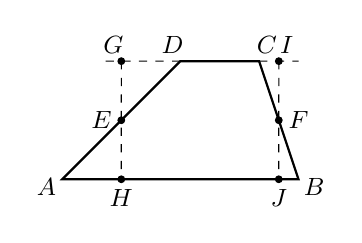
\begin{tikzpicture}[scale=1,font=\small]
\usetikzlibrary{calc}

\begin{scope}
\coordinate (a) at (0,0);
\coordinate (b) at (3,0);
\coordinate (c) at (2.5,1.5);
\coordinate (d) at (1.5,1.5);


\draw[thick] (a) node[shift={(-0.2,-0.1)}] {$A$} -- (b) node[shift={(0.2,-0.1)}] {$B$} -- (c) node[shift={(0.1,0.2)}] {$C$} -- (d) node[shift={(-0.1,0.2)}] {$D$} -- cycle;


\coordinate (e) at ($(a)!0.5!(d)$);
\coordinate (h) at ($(a)!(e)!(b)$);
\coordinate (f) at ($(b)!0.5!(c)$);
\coordinate (j) at ($(a)!(f)!(b)$);
\coordinate (g) at (intersection of h--e and c--d);
\coordinate (i) at (intersection of j--f and c--d);

\draw[dashed] (d) -- ($(d)!1.3!(g)$);
\draw[dashed] (c) -- ($(c)!2!(i)$);

\draw[dashed] (g) -- (h);
\draw[dashed] (i) -- (j);

\draw[fill] (e) circle (1.2pt) node[left] {$E$};
\draw[fill] (f) circle (1.2pt) node[right] {$F$};
\draw[fill] (g) circle (1.2pt) node[shift={(-0.1,0.2)}] {$G$};
\draw[fill] (i) circle (1.2pt) node[shift={(0.1,0.2)}] {$I$};
\draw[fill] (h) circle (1.2pt) node[below] {$H$};
\draw[fill] (j) circle (1.2pt) node[below] {$J$};

\end{scope}


\end{tikzpicture}

%	\caption{Esercizio~\ref{ese:7.1}}\label{fig:ese7.1}
%\end{figure}
\end{esercizio}
 
\begin{esercizio}
\label{ese:7.2}
Dai vertici $B$ e $C$ dell'ipotenusa di un triangolo rettangolo $ABC$ traccia le rette rispettivamente parallele ai cateti $AC$ e $AB$; sia $D$ il loro punto di intersezione. Dimostrare che $ABDC\doteq 2\cdot ABC$ e che $MNPQ\doteq 2\cdot ABC$ dove $MNPQ$ è il rettangolo avente un lato congruente all'ipotenusa $BC$ e l'altro lato congruente all'altezza $AH$ relativa all'ipotenusa.
\end{esercizio}

\begin{esercizio}
\label{ese:7.3}
Costruire un rettangolo equivalente ad un trapezio dato.
\end{esercizio}

\begin{esercizio}
\label{ese:7.4}
Dimostrare che la mediana relativa ad un lato di un triangolo divide il triangolo dato in due triangoli equivalenti.
\end{esercizio}

\begin{esercizio}
\label{ese:7.5}
Dimostrare che in un parallelogramma $ABCD$ sono equivalenti i quattro triangoli determinati dalle diagonali $AC$ e $BD$.
\end{esercizio}

\begin{esercizio}
\label{ese:7.6}
Assegnato il trapezio $ABCD$, detto $E$ il punto di intersezione delle diagonali $DB$ e $AC$, dimostrare che $DEA$ è equivalente a $BEC$.
\end{esercizio}

\begin{esercizio}
\label{ese:7.7}
Dimostra che le diagonali di un trapezio lo dividono in quattro triangoli due dei quali sono equiestesi.
\end{esercizio}

\begin{esercizio}
\label{ese:7.8}
Dimostra che due triangoli sono equiestesi se hanno due lati ordinatamente congruenti e gli angoli tra essi compresi supplementari.
\end{esercizio}

\begin{esercizio}
\label{ese:7.9}
Dimostra che un triangolo $ABC$ è diviso da una sua mediana in due triangoli equiestesi.
\end{esercizio}

\end{multicols}

\begingroup
\hypersetup{linkcolor=black}
\subsubsection*{\ref{sect:applicazioni_algebra} - \nameref{sect:applicazioni_algebra}}
\endgroup

\begin{multicols}{2}

\begin{esercizio}
\label{ese:7.10}
Sia $ABC$ un triangolo con $\overline{AB}=7$~cm, $\overline{BC}=5$~cm e $\overline{AC}=3$~cm. Condurre una parallela ad $AC$ che intersechi $AB$ in $D$ e $BC$ in $E$. Sapendo che $CE=BD$, trovare il perimetro del triangolo $BDE$.
\end{esercizio}

\begin{esercizio}
\label{ese:7.11}
Nel trapezio $ABCD$, le basi misurano 5~cm e 15~cm e l'area vale 120~cm\textsuperscript{2}. Determina la distanza tra la base maggiore ed il punto di intersezione dei lati obliqui del trapezio.
\end{esercizio}

\begin{esercizio}
\label{ese:7.12}
Sia $ABC$ un triangolo rettangolo in $A$, con $AB=8a$. Da un punto $D$ di $AC$ si tracci la parallela ad $AB$ che incontri $BC$ in $E$; sia $DE=6a$. Sapendo che $CDE$ e $ABED$ sono isoperimetrici, trovare l'area di $ABC$.
\end{esercizio}

\begin{esercizio}
\label{ese:7.13}
Nel trapezio rettangolo $ABCD$ circoscritto ad una circonferenza  la base maggiore è $4/3$ dell'altezza ed il perimetro misura 48~cm. Trovare l'area del trapezio.
\end{esercizio}

\begin{esercizio}
\label{ese:7.14}
Sia $ABC$ un triangolo rettangolo in $A$ con il cateto $AC = 32a$. Sapendo che $BC:AB=5:3$, trovare il perimetro del triangolo. Tracciare poi la parallela ad $AB$, che intersechi $CA$ in $D$ e $CB$ in $E$. Sapendo che $CD$ è medio proporzionale tra $CE$ ed $AB$, trovare l'area del trapezio $ABED$.
\end{esercizio}

\begin{esercizio}
\label{ese:7.15}
Sia $ABC$ un triangolo isoscele di base $BC=4$~cm e di area 40~cm\textsuperscript{2}. Dopo aver trovato la misura dell'altezza $AH$ si tracci l'altezza $CK$ e la si prolunghi di un segmento $KD$ tale che l'angolo $H\widehat{A}D$ sia congruente ad uno degli angoli alla base. Dopo aver dimostrato che $C\widehat{A}D$ è retto, trovare il perimetro del triangolo $CAD$.
\end{esercizio}

\begin{esercizio}
\label{ese:7.16}
Due lati consecutivi di un parallelogramma misurano $2a$ e $4a$ e l'angolo tra essi compreso misura $60\grado$. Trovare la misura dell'area e delle diagonali.
\end{esercizio}

\begin{esercizio}
\label{ese:7.17}
Determinare perimetro ed area di un trapezio rettangolo circoscritto ad una circonferenza, sapendo che il lato obliquo è diviso dal punto di tangenza in due parti che misurano rispettivamente $4a$ e $9a$.
\end{esercizio}

\begin{esercizio}
\label{ese:7.18}
Determinare perimetro ed area di un triangolo isoscele, sapendo che la base misura $10a$ e che l'angolo adiacente ad uno degli angoli alla base misura $150\grado$.
\end{esercizio}

\begin{esercizio}
\label{ese:7.19}
Nel trapezio $ABCD$ la base maggiore, $AB$, misura 15~cm e la minore, $CD$, misura 5~cm. Prolungando i lati obliqui si ottiene un triangolo rettangolo. Trovare il perimetro del trapezio e del triangolo rettangolo $CDE$ sapendo che la differenza tra le due basi è uguale alla differenza tra il doppio di $BC$ e $AD$.
\end{esercizio}

\begin{esercizio}[Giochi di Archimede 2011]
\label{ese:7.20}
In un triangolo equilatero $ABC$ con lato di lunghezza 3~m, prendiamo i punti $D$, $E$ e $F$ sui lati $AC$, $AB$ e $BC$ rispettivamente, in modo che i segmenti $AD$ e $FC$ misurino 1~m e il segmento $DE$ sia perpendicolare ad $AC$. Quanto misura l'area del triangolo $DEF$?
\end{esercizio}

\begin{esercizio}
\label{ese:7.21}
\`E dato un trapezio isoscele avente un angolo di $45\grado$ e il lato obliquo che misura 2~cm. Trovare l'area sapendo che la base minore misura $\sqrt{3}$~cm.
\end{esercizio}

\begin{esercizio}
\label{ese:7.22}
Nella circonferenza di diametro $BD$ sono inscritti i triangoli $ABD$ e $BDC$, con $A$ e $C$ da parti opposte rispetto a $BD$. Sia $H$ la proiezione di $C$ su $BD$. Sapendo che $AB=16$~cm e che il rapporto tra $AD$ e $BD$ e tra $BH$ e $HD$ è $3/5$, trovare il perimetro di $ABCD$.
\end{esercizio}

\begin{esercizio}
\label{ese:7.23}
Il quadrato $ABCD$ ha il lato di 2~m; costruite sul lato $DC$ il triangolo isoscele $DEC$ di base $DC$ e avente $D\widehat{E}C=120\grado$; siano $F$ e $G$ i punti di intersezione delle rette $ED$ e $EC$ con la retta $AB$. Determinate la misura dei lati del triangolo $EFG$.
\end{esercizio}

\begin{esercizio}
\label{ese:7.24}
\`E dato il triangolo equilatero $ABC$; la semiretta $r$ di origine $B$ è interna all'angolo $ABC$ e lo divide in due parti di cui $ABP=45\grado$, $P0r\cap AC$. Sapendo che la distanza di $P$ dal lato $AB$ è di 2~m, calcolate il perimetro del triangolo equilatero dato.
\end{esercizio}

\begin{esercizio}
\label{ese:7.25}
Su ciascun lato del triangolo equilatero $ABC$ costruite un quadrato. Sapendo che l'altezza del triangolo equilatero misura $3\sqrt{3}$~m, determinate il perimetro e l'area dell'esagono che si forma congiungendo i vertici dei quadrati. Costruite il rettangolo equivalente all'esagono.
\end{esercizio}

\begin{esercizio}
\label{ese:7.26}
Nel trapezio rettangolo $ABCD$ di base maggiore $AB$, l'angolo acuto di vertice $B$ misura $45\grado$ e l'altezza è di 8~m. Sapendo che la base minore è $3/4$ dell'altezza, determinate perimetro e area del trapezio.
\end{esercizio}

\begin{esercizio}
\label{ese:7.27}
Nel parallelogramma $ABCD$ la diagonale minore $AC$ è perpendicolare al lato $BC$ e forma col lato $AB$ un angolo di $45\grado$. Sapendo che $AC=5$~m, calcolate il perimetro e l'area del parallelogramma.
\end{esercizio}

\begin{esercizio}
\label{ese:7.28}
Il trapezio $ABCD$ di base maggiore $AB$, ha $\widehat{A}=45\grado$ e $\widehat{B}=60\grado$; sapendo che la base minore è uguale all'altezza che misura 12~cm, determinate perimetro e area del trapezio.
\end{esercizio}

\begin{esercizio}
\label{ese:7.29}
Il quadrilatero $ABCD$ è spezzato dalla diagonale $AC$ nel triangolo rettangolo isoscele $ABC$ retto in $B$ e nel triangolo $ADC$ isoscele su $AC$, avente l'altezza $DH$ doppia della base. Sapendo che $AB=5$~m, calcolate il perimetro e l'area del quadrilatero.
\end{esercizio}

\begin{esercizio}
\label{ese:7.30}
Il triangolo isoscele $ABC$ ha l'angolo in $A$ opposto alla base $BC$ di $120\grado$ ed è circoscritto ad una circonferenza di raggio $OH=\sqrt{6}$~m; calcolate perimetro e area del triangolo dato.
\end{esercizio}

\begin{esercizio}
\label{ese:7.31}
Nel triangolo $ABC$ l'angolo in $A$ misura $60\grado$ e sia $AE$ la sua bisettrice ($E$ su $BC$). Sapendo che $AE=8$~m, determinate la misura delle distanze $EH$ ed $EK$ del punto $E$ rispettivamente dai lati $AB$ e $AC$ e il perimetro del quadrilatero $AHEK$. \`E vero che tale quadrilatero è equivalente al triangolo equilatero di lato 8~m? \`E vero che tale quadrilatero può essere inscritto in una circonferenza? Se la risposta è affermativa stabilite il suo centro e determinate la misura di detta circonferenza.
\end{esercizio}

\begin{esercizio}
\label{ese:7.32}
Nel trapezio rettangolo $ABCD$ la base minore è metà dell'altezza. Determinate perimetro e area in funzione della misura $x$ della base minore nei casi in cui l'angolo acuto del trapezio è di
\begin{enumeratea}
\item $45\grado$;
\item $30\grado$;
\item $60\grado$.
\end{enumeratea}
\end{esercizio}

\begin{esercizio}
\label{ese:7.33}
Il triangolo $ABC$ è rettangolo e l'angolo di vertice $C$ misura $30\grado$; detta $AP$ la bisettrice dell'angolo retto, con $P$ su $BC$, e sapendo che $\overline{AP}=a$, determinate, in funzione di $a$, perimetro e area del triangolo dato.
\end{esercizio}

\begin{esercizio}
\label{ese:7.34}
Il segmento $AC$ è la diagonale del quadrilatero $ABCD$ avente $A\widehat{B}C=C\widehat{A}D=90\grado$ e $B\widehat{C}A=A\widehat{D}C=60\grado$. \`E vero che $ABCD$ è un trapezio rettangolo? Calcolate perimetro e area del quadrilatero sapendo che $\overline{AC}=2a$.
\end{esercizio}

\begin{esercizio}
\label{ese:7.35}
Il quadrato $ABCD$ ha i suoi vertici sui lati del triangolo equilatero $HKL$ ($A$ e $B$ appartengono a $KL$, $C$ a $HL$ e $D$ a $HK$); sapendo che $\overline{AB}=3a$, calcolate il perimetro e l'area del triangolo equilatero.
\end{esercizio}

\begin{esercizio}
\label{ese:7.36}
In un parallelogramma di area 12~m\textsuperscript{2}, le lunghezze di due lati consecutivi sono una il doppio dell'altra e uno degli angoli interni misura $60\grado$. Determina la lunghezza delle diagonali.
\end{esercizio}

\begin{esercizio}
\label{ese:7.37}
Nel triangolo $ABC$ di altezza $CH=8$~m, determina a quale distanza da $C$ si deve condurre una parallela al lato $AB$ in modo che il triangolo ottenuto sia equivalente alla metà di $ABC$.
\end{esercizio}

\begin{esercizio}
\label{ese:7.38}
La base di un rettangolo è più lunga di 8~cm dell'altezza ed è più corta di 10~cm della diagonale. Calcola la base del rettangolo. 			
\end{esercizio}

\begin{esercizio}
\label{ese:7.39}
In un triangolo equilatero $ABC$ di lato 1 individua sul lato $AB$ un punto $P$ tale che detti $H$ e $K$ i piedi delle perpendicolari condotte da $P$ ai lati $AC$ e $BC$ risulti $\overline{PH}^2+\overline{PK}^2=\overline{PC}^2+\np{12,67}$
\end{esercizio}

\begin{esercizio}
\label{ese:7.40}
Un triangolo equilatero e un quadrato hanno lo stesso perimetro. Quanto vale il rapporto tra le aree delle due figure?
\end{esercizio}

\begin{esercizio}
\label{ese:7.41}
In un triangolo rettangolo $ABC$, retto in $A$, si tracci una parallela $DE$ al cateto $AB$. Sapendo che l'area di $DEC$ è i $3/4$ di quella di $ABC$ e che $\overline{AC}$ misura 1~m, quanto misura $\overline{DC}$?
\end{esercizio}

\begin{esercizio}
\label{ese:7.42}
Dato il quadrato $ABCD$ con $M$ punto medio di $AB$ ed $N$ punto medio di $CD$, tracciare i segmenti $AN$, $BN$, $DM$ e $CM$. Siano $P$ l'intersezione di $AN$ con $DM$ e $Q$ l'intersezione di $BN$ e $CM$. Che figura è $MQNP$? Quanti triangoli ci sono nella figura? Calcolare l'area di $MQNP$ e l'area di uno dei triangoli ottusangoli, sapendo che il lato del quadrato è 12~cm.
\end{esercizio}

\begin{esercizio}
\label{ese:7.43}
Disegna un rombo con la diagonale minore lunga 6~cm e la diagonale maggiore 8~cm. Costruisci su ciascun lato del rombo un quadrato. Unisci i vertici liberi dei quadrati formando un ottagono. Calcolane l'area. Calcola anche l'area dei quattro triangoli che si sono formati. Calcola inoltre la misura degli angoli interni dell'ottagono.
\end{esercizio}

\begin{esercizio}
\label{ese:7.44}
Disegna un quadrato $ABCD$ e sul lato $AB$ poni i punti $M$ ed $N$ in modo che $AM\cong MN\cong NB$. Che figura è $MNCD$? Calcola il rapporto tra l'area di $MNCD$ e quella di $ABCD$. Calcola il perimetro di $MNCD$ sapendo che l'area del quadrato è 10~cm\textsuperscript{2}.
\end{esercizio}

\begin{esercizio}
\label{ese:7.45}
Disegna un triangolo isoscele $ABC$ di base $AC=40$~mm e lato obliquo $AB=52$~mm. Costruisci sulla base $AC$ il triangolo $ACD$ di area doppia di $ABC$ e determina il perimetro del quadrilatero $ABCD$. Di che figura si tratta?
\end{esercizio}

\begin{esercizio}
\label{ese:7.46}
Il parallelogramma $ABCD$ ha la base $AB$ lunga 12~cm e l'altezza di 6~cm. Disegna su $AB$ un punto $H$ e su $CD$ un punto $K$ tali che $DK=BH=3$~cm. Considera i due quadrilateri in cui il parallelogramma rimane diviso dal segmento $HK$: che quadrilateri sono? Calcolane l'area. Calcola inoltre il rapporto tra l'area di $HBCD$ e quella di $ABCD$.
\end{esercizio}

\begin{esercizio}
\label{ese:7.47}
Calcola l'altezza del rombo avente le diagonali di 36~cm e 48~cm. Calcola l'area del trapezio equivalente al rombo, sapendo che l'altezza del trapezio è di 24~cm e che la base maggiore è il doppio di quella minore.
\end{esercizio}

\begin{esercizio}
\label{ese:7.48}
Il rettangolo $R$ ha base $AB = 9$~cm e l'altezza $BC$ è i $4/3$ di $AB$. Calcola il perimetro e l'area di $R$. Disegna il parallelogramma $P$ equivalente al rettangolo $R$ e avente la base congruente alla diagonale del rettangolo. Calcola l'altezza di $P$.
\end{esercizio}

\begin{esercizio}
\label{ese:7.49}
Calcola l'area del parallelogramma $P$ di base \np{4,5}~cm e altezza 2~cm e con il lato obliquo che è $5/4$ dell'altezza. Disegna la diagonale $AC$ e traccia l'altezza relativa ad $AB$ del triangolo $ABC$. Calcola l'area del triangolo $ABC$.
\end{esercizio}

\begin{esercizio}
\label{ese:7.50}
I lati del triangolo $ABC$ hanno le seguenti misure $AB=21$~cm, $BC=20$~cm e $AC=13$~cm; calcola l'area del parallelogramma $A'B'C'D'$ di base $AB\cong A'B'$, lato $AC\cong A'C'$ e diagonale $B'C'\cong BC$ (ricorda la formula di Erone).
\end{esercizio}

\begin{esercizio}
\label{ese:7.51}
Dato il rombo $ABCD$, avente perimetro di 10~cm e la diagonale maggiore di 4~cm, calcola la misura della diagonale minore, l'area del rombo e la sua altezza. Considera un triangolo isoscele equivalente al rombo e avente la sua stessa altezza. Calcolane la misura di ciascun lato.
\end{esercizio}

\begin{esercizio}
\label{ese:7.52}
Un rombo ha l'area di 336~cm\textsuperscript{2}, una diagonale uguale alla base di un triangolo di altezza \np{20,2}~cm e area di \np{141,4}~cm\textsuperscript{2}. Determina il perimetro del rombo.
\end{esercizio}

\begin{esercizio}
\label{ese:7.53}
Determina l'area del quadrato formato dai 4 vertici liberi di 4 triangoli equilateri costruiti sui lati di un quadrato di lato 3~cm.
\end{esercizio}

\begin{esercizio}
\label{ese:7.54}
Determina l'area del rombo intersezione di due triangoli equilateri costruiti sui lati opposti di un quadrato di lato 10~cm e aventi il vertice che cade internamente al quadrato.
\end{esercizio}

\begin{esercizio}
\label{ese:7.55}
Determina le misure degli angoli del triangolo $AED$ formato disegnando le diagonali $EA$ e $AD$ di un esagono regolare $ABCDEF$.
\end{esercizio}

\begin{esercizio}
\label{ese:7.56}
Determina le misure degli angoli del triangolo $AEC$ formato disegnando le diagonali $EA$ ed $EC$ di un ottagono regolare $ABCDEFGH$.
\end{esercizio}

\begin{esercizio}
\label{ese:7.57}
Determina le misure degli angoli del triangolo $AFC$ formato disegnando le diagonali $AF$ e $FC$ di un ottagono regolare $ABCDEFGH$.
\end{esercizio}

\begin{esercizio}
\label{ese:7.58}
La differenza tra le diagonali di un rombo è 7~cm e una è $5/12$ dell'altra. Determina l'area di un triangolo isoscele il cui perimetro supera di 6~cm quello del rombo e la cui base è 8~cm.
\end{esercizio}

\begin{esercizio}
\label{ese:7.59}
Determinare l'area di un quadrilatero con le diagonali perpendicolari sapendo che l'una è $5/8$ dell'altra e che la loro somma è 39~cm.
\end{esercizio}

\begin{esercizio}
\label{ese:7.60}
Determinare la misura degli angoli di un parallelogramma sapendo che uno degli angoli alla base è $2/7$ di quello adiacente.
\end{esercizio}

\begin{esercizio}
\label{ese:7.61}
In un quadrilatero un angolo è $93\grado8'42''$. Determinare l'ampiezza di ciascuno degli altri tre angoli sapendo che il secondo è $2/7$ del terzo e il terzo è $4/5$ del quarto.
\end{esercizio}

\begin{esercizio}
\label{ese:7.62}
Le dimensioni $a$ e $b$ di un rettangolo sono $a=\frac{3}{5}b$, il perimetro è 192~cm. Calcolane l'area.
\end{esercizio}

\begin{esercizio}
\label{ese:7.63}
In un rombo la differenza fra le diagonali è 8~cm e una diagonale è i $4/3$ dell'altra. Calcola area e perimetro del rombo.
\end{esercizio}

\begin{esercizio}
\label{ese:7.64}
In un rombo la somma delle diagonali misura 196~cm, un quarto della misura della diagonale maggiore supera di 4~cm la misura della diagonale minore. Trova perimetro, area e altezza del rombo.
\end{esercizio}

\begin{esercizio}
\label{ese:7.65}
In un trapezio rettangolo l'altezza è quadrupla della base minore e il lato obliquo è i $5/4$ dell'altezza. Determina l'area del trapezio sapendo che il suo perimetro è 70~cm.
\end{esercizio}

\begin{esercizio}
\label{ese:7.66}
Il perimetro di un trapezio isoscele misura 124~cm e ciascun lato obliquo è lungo 30~cm. Determinane l'area e la misura della diagonale sapendo che una sua base è $7/25$ dell'altra.
\end{esercizio}

\begin{esercizio}
\label{ese:7.67}
Determina l'area di un rettangolo sapendo che la misura della sua diagonale supera di 8~cm quella dell'altezza e che la differenza fra i $20/41$ della diagonale ed i $2/3$ dell'altezza è uguale ai $14/9$ della stessa altezza.
\end{esercizio}

\begin{esercizio}
\label{ese:7.68}
Il perimetro di un rettangolo misura 170~cm e l'altezza è $5/12$ della base. Trovare area e diagonale del rettangolo.
\end{esercizio}

\begin{esercizio}
\label{ese:7.69}
Il perimetro di un rettangolo misura 29~cm ed i $2/11$ della sua altezza sono uguali a $1/9$ della base. Trovare l'area del rettangolo.
\end{esercizio}

\begin{esercizio}
\label{ese:7.70}
In un trapezio isoscele $ABCD$ avente la base maggiore $AB$, le diagonali sono fra loro perpendicolari e si intersecano in un punto $P$ che divide ogni diagonale in due parti con rapporto $5/12$. Calcola perimetro e area del trapezio, sapendo che la diagonale misura 68~cm.
\end{esercizio}

\begin{esercizio}
\label{ese:7.71}
Un triangolo rettangolo ha ipotenusa 50~cm e un cateto 48~cm. Dal punto medio dell'ipotenusa tracciare la parallela al cateto minore. Determinare l'area di ciascuna delle due parti in cui è suddiviso il triangolo.
\end{esercizio}

\begin{esercizio}
\label{ese:7.72}
In un triangolo l'altezza è 18~cm; se conducendo una parallela alla base, si divide il triangolo in due parti la cui superficie è in rapporto $16/25$, a quale distanza dal vertice è stata condotta la parallela?
\end{esercizio}

\begin{esercizio}
\label{ese:7.73}
Il triangolo $ABC$ ha base 14~cm e altezza 6~cm. Disegna la mediana $CM$ e calcola l'area dei triangoli $AMC$ e $MBC$. Come sono i triangoli?
\end{esercizio}

\begin{esercizio}
\label{ese:7.74}
La mediana di un triangolo è 12~cm. Determinare la misura di ciascuna delle parti in cui il baricentro divide la mediana.
\end{esercizio}

\begin{esercizio}
\label{ese:7.75}
Determinare la misura di una mediana $AM$ sapendo che $BM=8$~cm, dove $B$ è il baricentro del triangolo.
\end{esercizio}

\begin{esercizio}
\label{ese:7.76}
Determina la misura $BM$ del segmento appartenente alla mediana $AM$ in un triangolo equilatero $ABC$, avendo indicato con $B$ il baricentro. 
\end{esercizio}

\begin{esercizio}
\label{ese:7.77}
Determina il perimetro di un triangolo rettangolo sapendo che l'altezza relativa all'ipotenusa è 8~cm e che la proiezione di un cateto sull'ipotenusa è $4/3$ dell'altezza data.
\end{esercizio}

\begin{esercizio}
\label{ese:7.78}
Determina la misura delle tre altezze del triangolo che ha i lati di 20~cm, 40~cm, 30~cm. (Suggerimento: Puoi ricorrere alla formula di Erone).
\end{esercizio}

\begin{esercizio}
\label{ese:7.79}
Il piede dell'altezza $CH$ di un triangolo $ABC$ divide la base $AB$ di 46~cm in due parti tali che $AH=\dfrac{9}{14}HB$; calcola l'area dei due triangoli $ACH$ e $BCH$, sapendo che $AC=24$~cm.
\end{esercizio}

\begin{esercizio}
\label{ese:7.80}
Trova il perimetro di un triangolo isoscele sapendo che la base è $2/3$ dell'altezza e che l'area è 24~cm\textsuperscript{2}.
\end{esercizio}

\begin{esercizio}
\label{ese:7.81}
Trova il perimetro di un triangolo isoscele sapendo che la base è $3/5$ dell'altezza e che l'area è 24~cm\textsuperscript{2}.
\end{esercizio}

\begin{esercizio}
\label{ese:7.82}
I lati del triangolo $ABC$ hanno le misure seguenti $AB=63$~cm, $BC=60$~cm e $AC=39$~cm; determina le misure delle tre relative altezze.
\end{esercizio}

\begin{esercizio}
\label{ese:7.83}
Determinare la misura di ciascun lato e l'area del triangolo isoscele avente il perimetro di 700~m, sapendo che la base e il lato obliquo sono in rapporto $\frac{16}{17}$.
\end{esercizio}

\begin{esercizio}
\label{ese:7.84}
Un trapezio rettangolo $ABCD$ è circoscritto ad una semicirconferenza con il centro $O$ sulla sua base maggiore $AB$ e raggio di misura 6~cm. Siano $S$ e $T$ i punti in cui tale semicirconferenza tange rispettivamente il lato obliquo $BC$ e la base minore $CD$. Sapendo che $AB$ misura 16~cm, calcolare le misure degli altri lati del trapezio. (Tracciare $OC$, $OS$, $OT$ e dimostrare che $OB$ è congruente a \ldots{}).
\end{esercizio}

\begin{esercizio}
\label{ese:7.85}
Calcolare perimetro e area di un triangolo isoscele circoscritto a una semicirconferenza con il centro sulla sua base, sapendo che la base è i $3/2$ della relativa altezza e che il raggio della semicirconferenza misura 12~cm.
\end{esercizio}

\begin{esercizio}
\label{ese:7.86}
Data una circonferenza di centro $O$, si consideri un punto $C$ esterno ad essa da cui si traccino le tangenti alla circonferenza stessa indicando con $A$ e $B$ i punti di tangenza. Sapendo che il segmento $AB$ misura 12~cm e che l'angolo $A\widehat{C}B$ ha ampiezza $60\grado$, calcolare il perimetro e l'area del quadrilatero $OACB$. Indicato poi con $E$ il punto in cui la retta $OB$ incontra la retta $AC$, calcolare il perimetro del triangolo $BCD$.
\end{esercizio}

\begin{esercizio}
\label{ese:7.87}
In un trapezio rettangolo, l'angolo che il lato obliquo forma con la base maggiore ha ampiezza $60\grado$ e la diagonale maggiore dimezza tale angolo; sapendo che la base minore misura 4~cm,  calcolare il perimetro del trapezio.
\end{esercizio}

\begin{esercizio}
\label{ese:7.88}
In un rombo $ABCD$ ciascun lato misura 12~cm e l'angolo in $B$ ha ampiezza $120\grado$. Prendere sui lati $AB$, $BC$, $CD$ e $AD$ del rombo rispettivamente i punti $P$, $Q$, $S$ e $T$ in modo che i segmenti $AP$, $BQ$, $CS$ e $DT$ misurino 2~cm ciascuno. Calcolare il perimetro e l'area del quadrilatero $PQST$, dopo aver dimostrato che esso è un parallelogramma. (Tracciare da $T$ il segmento perpendicolare ad $AB$ e osservare i vari triangoli \ldots{}, analogamente tracciare poi da $P$ il segmento perpendicolare alla retta \ldots{}).  
\end{esercizio}

\begin{esercizio}
\label{ese:7.89}
Sul lato $AB$ di un triangolo equilatero $ABC$ avente area uguale a $25\sqrt{3}$~cm\textsuperscript{2}, si prenda il punto $P$ in modo che $AP$ misuri 4~cm; si tracci il segmento $PQ$ parallelo a $BC$ (con $Q$ appartenente ad $AC$) e lo si prolunghi di un segmento $QE$ congruente a $PQ$. Dopo aver dimostrato che il triangolo $APE$ è rettangolo, calcolare perimetro ed area del quadrilatero $CEPH$, essendo $H$ il piede dell'altezza del triangolo $ABC$ relativa ad $AB$.
\end{esercizio}

\begin{esercizio}
\label{ese:7.90}
Data una semicirconferenza di centro $O$ e diametro $AB$ di misura $2r$, si tracci la corda $AC$ che forma con $AB$ un angolo di $30\grado$; si tracci quindi la tangente in $C$ alla semicirconferenza indicando con $D$ il punto in cui tale tangente incontra la retta $AB$ e con $E$ la proiezione ortogonale di $B$ sulla tangente stessa. Calcolare le misure dei segmenti $BC$, $CD$, $BE$, $CE$, $AE$. (Tracciare anche $CO$ \ldots{} osservare i vari angoli; per calcolare la misura di $AE$ tracciare la distanza di \ldots{} dalla retta \ldots{}).
\end{esercizio}

\begin{esercizio}
\label{ese:7.91}
Determina area e perimetro del quadrilatero $ABCD$ di coordinate $A(-1;7)$, $B(6;9/2)$, $C(4;-3)$ e $D(-4;3)$.
\end{esercizio}

\begin{esercizio}
\label{ese:7.92}
Determina area a perimetro del quadrilatero $ABCD$ di coordinate $A(0;3)$, $B(3;6)$, $C(6;3)$ e $D(-4;3)$. Che quadrilatero è?
\end{esercizio}

\begin{esercizio}
\label{ese:7.93}
Determina l'area del quadrilatero $ABCD$ di coordinate $A(-8;5)$, $B(-2;11)$, $C(2;12)$ e $D(4;3)$.
\end{esercizio}

\begin{esercizio}
\label{ese:7.94}
Determina il quarto vertice $D$ del trapezio $ABCD$ di area $9$, sapendo che $A(-1;2)$, $B(5;2)$ e $C(3;4)$.
\end{esercizio}

\begin{esercizio}
\label{ese:7.95}
Determina il quarto vertice $D$ del parallelogramma $ABCD$ con $A(-3;-1)$, $B(4;1)$ e $C(3;4)$.
\end{esercizio}

\begin{esercizio}
\label{ese:7.96}
Verifica che il trapezio di vertici $A(-1;-1)$, $B(3;-2)$, $C\left(3;\frac{1}{2}\right)$ e $D\left(0;\frac{5}{2}\right)$ non è rettangolo. Calcola l'intersezione $E$ dei prolungamenti dei lati obliqui $BC$ e $AD$. Calcola inoltre il rapporto tra le aree dei triangoli $ABE$ e $CDE$.
\end{esercizio}

\begin{esercizio}
\label{ese:7.97}
Verifica che il quadrilatero di vertici $A(-2;-3)$, $B(3;-2)$, $C(4;1)$ e $D(0;3)$ è un trapezio e calcolane l'altezza.
\end{esercizio}

\begin{esercizio}
\label{ese:7.98}
Verifica che il quadrilatero di vertici $A(-4;1)$, $B(5;-2)$, $C(3;2)$ e $D(0;3)$ è un trapezio isoscele. Calcola l'intersezione $E$ dei prolungamenti dei lati obliqui $BC$ e $AD$. Calcola inoltre il rapporto tra le aree dei triangoli $ABE$ e $CDE$.
\end{esercizio}

\begin{esercizio}[Giochi di Archimede 2011]
\label{ese:7.99}
Nel quadrilatero $ABCD$ le diagonali sono ortogonali tra loro e gli angoli in $B$ e in $D$ sono retti. Inoltre $AB=AD=20$~cm e $BC=CD=30$~cm. Calcolare il raggio della circonferenza inscritta in $ABCD$.
\end{esercizio}

\begin{esercizio}[Giochi di Archimede 2003]
\label{ese:7.100}
Sia dato un quadrato $ABCD$ di lato unitario e sia $P$ un punto interno ad esso tale che l'angolo $A\widehat{P}B$ misuri $75\grado$. Quanto vale la somma delle aree dei triangoli $ABP$ e $CDP$? 
\end{esercizio}

\begin{esercizio}[Giochi di Archimede 2003]
\label{ese:7.101}
Un parallelogramma di lati 1 e 2 ha un angolo di $60\grado$. Quanto misura la sua diagonale minore?   
\end{esercizio}

\begin{esercizio}[Giochi di Archimede 2007]
\label{ese:7.102}
In un triangolo $ABC$ scegliamo un punto $D$ su $AB$ e un punto $E$ su $AC$ in modo che la lunghezza di $AD$ sia un terzo di quella di $AB$ e la lunghezza di $AE$ sia un terzo di quella di $AC$. Sapendo che l'area del triangolo $ADE$ è 5~m\textsuperscript{2}, determinare l'area del quadrilatero $BCED$.
\end{esercizio}

\begin{esercizio}[Giochi di Archimede 2007]
\label{ese:7.103}
Il quadrato $ABCD$ ha il lato lungo 3~m. Il segmento $EF$ è lungo 1~m ed è parallelo ad $AB$. Quanto vale l'area dell'esagono $ABFCDE$?
\end{esercizio}

%\begin{figure}[!htb]
	\centering% Copyright (c) 2015 Daniele Masini - d.masini.it@gmail.com

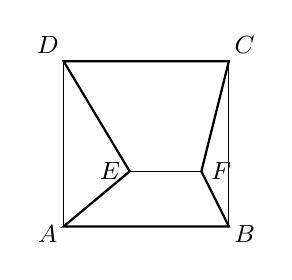
\begin{tikzpicture}[scale=0.7,font=\small]
\usetikzlibrary{calc}

\begin{scope}
\coordinate (a) at (0,0);
\coordinate (b) at (3,0);
\coordinate (c) at (3,3);
\coordinate (d) at (0,3);
\coordinate (e) at (1.2,1);
\coordinate (f) at (2.5,1);

\draw[thick] (a) node[shift={(-0.2,-0.1)}] {$A$} -- (b) node[shift={(0.2,-0.1)}] {$B$} -- (f) node[shift={(0.25,0)}] {$F$} -- (c) node[shift={(0.2,0.2)}] {$C$} -- (d) node[shift={(-0.2,0.2)}] {$D$} -- (e) node[shift={(-0.25,0)}] {$E$} -- cycle;
\draw (a) -- (d);
\draw (b) -- (c);
\draw (e) -- (f);

\end{scope}


\end{tikzpicture}

%	\caption{Esercizio~\ref{ese:7.104}}\label{fig:ese7.104}
%\end{figure}

\begin{esercizio}[Giochi di Archimede 2007]
\label{ese:7.104}
$ABCD$ è un quadrato avente la diagonale lunga 2~cm e $AEC$ è equilatero. Quanto vale l'area del quadrilatero $AECB$?
\end{esercizio}

%\begin{figure}[!htb]
	\centering% Copyright (c) 2015 Daniele Masini - d.masini.it@gmail.com

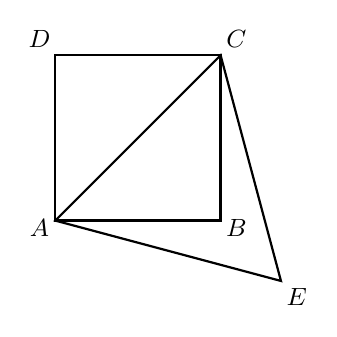
\begin{tikzpicture}[scale=0.7,font=\small]
\usetikzlibrary{calc, intersections}

\begin{scope}
\clip (-0.5,-1.6) rectangle (4.6,3.5);
\coordinate (a) at (0,0);
\coordinate (b) at (3,0);
\coordinate (c) at (3,3);
\coordinate (d) at (0,3);

\path[name path = Circle1] (a) let \p1 = ($(c)-(a)$) in circle ({veclen(\x1,\y1)});
\path[name path = Circle2] (c) let \p1 = ($(a)-(c)$) in circle ({veclen(\x1,\y1)});
\path [name intersections={of=Circle1 and Circle2}];
\path (intersection-2) coordinate (e) node[shift={(0.2,-0.2)}] {$E$};

\draw[thick] (a) node[shift={(-0.2,-0.1)}] {$A$} -- (b) node[shift={(0.2,-0.1)}] {$B$} -- (c) node[shift={(0.2,0.2)}] {$C$} -- (d) node[shift={(-0.2,0.2)}] {$D$} -- cycle;
\draw[thick] (a) -- (c) -- (e) -- cycle;

\end{scope}


\end{tikzpicture}

%	\caption{Esercizio~\ref{ese:7.105}}\label{fig:ese7.105}
%\end{figure}

\begin{esercizio}[Giochi d'Autunno 2010]
\label{ese:7.105}
Da un quadrato di lato 10~cm si tagliano i quattro angoli in modo da ottenere un ottagono regolare. Quanto è lungo il lato dell'ottagono?
\end{esercizio}

%\begin{figure}[!htb]
	\centering% (c) 2014 Daniele Masini - d.masini.it@gmail.com
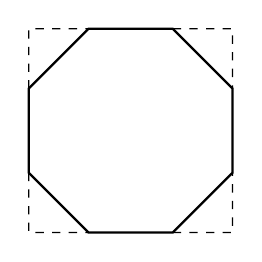
\begin{tikzpicture}[scale=0.7,font=\small]
\usetikzlibrary{calc}
\pgfmathsetmacro{\lati}{8}
\pgfmathsetmacro{\angoloc}{360/\lati}

\begin{scope}[rotate={\angoloc/2-90}]
\coordinate (o) at (0,0);

\foreach \x/\y in {0/A,1/B,2/C,3/D,4/E,5/F,6/G,7/H}
{
	\path +({\x*\angoloc}:2) coordinate (\y) -- ({(\x+1)*\angoloc}:2);
}
\draw[thick] (A) -- (B) -- (C) -- (D) -- (E) -- (F) -- (G) -- (H) -- cycle; 

\end{scope}

\coordinate (ef) at (intersection of D--E and G--F);
\coordinate (cd) at (intersection of D--E and C--B);
\coordinate (ab) at (intersection of C--B and A--H);
\coordinate (gh) at (intersection of A--H and F--G);

\draw[dashed] (F) -- (ef) -- (E);
\draw[dashed] (D) -- (cd) -- (C);
\draw[dashed] (A) -- (ab) -- (B);
\draw[dashed] (G) -- (gh) -- (H);

\end{tikzpicture}

%	\caption{Esercizio~\ref{ese:7.106}}\label{fig:ese7.106}
%\end{figure}

\begin{esercizio}[Giochi di Archimede 2006]
\label{ese:7.106}
Il segmento $DE$ è parallelo ad $AB$. Sapendo che l'area di $DEC$ è uguale ai $3/4$ di quella di $ABC$ e che $AC$ misura 1~m, quanto misura $DC$?
\end{esercizio}

%\begin{figure}[!htb]
	\centering% (c) 2014 Daniele Masini - d.masini.it@gmail.com
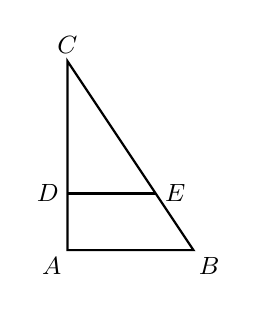
\begin{tikzpicture}[scale=0.8,font=\small]
\usetikzlibrary{calc}

\begin{scope}
%\clip (-2.1,-2.1) rectangle (2.5,2.1);
\coordinate (a) at (0,0);
\coordinate (b) at (2,0);
\coordinate (c) at (0,3);

\draw[thick] (a) node[shift={(-0.2,-0.2)}] {$A$} -- (b) node[shift={(0.2,-0.2)}] {$B$} -- (c) node[shift={(0,0.2)}] {$C$} -- cycle;

\draw[thick] ($(c)!0.7!(a)$) node[shift={(-0.25,0)}] {$D$} -- ($(c)!0.7!(b)$) node[shift={(0.25,0)}] {$E$};

\end{scope}


\end{tikzpicture}

%	\caption{Esercizio~\ref{ese:7.107}}\label{fig:ese7.107}
%\end{figure}

\begin{esercizio}[Giochi di Archimede 2005]
\label{ese:7.107}
Il triangolo $ABC$ è rettangolo ed i cateti $AB$ e $AC$ misurano rispettivamente 3~m e 4~m. Siano $B'$ e $C'$ punti appartenenti rispettivamente ai lati $AB$ e $AC$, tali che la retta contenente il segmento $B'C'$ sia parallela a quella contenete il segmento $BC$ e distante 1~m da essa. Calcolare l'area del triangolo $AB'C'$.
\end{esercizio}

%\begin{figure}[!htb]
	\centering% Copyright (c) 2015 Daniele Masini - d.masini.it@gmail.com

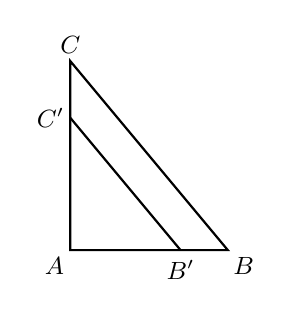
\begin{tikzpicture}[scale=0.8,font=\small]
\usetikzlibrary{calc}

\begin{scope}
%\clip (-2.1,-2.1) rectangle (2.5,2.1);
\coordinate (a) at (0,0);
\coordinate (b) at (2.5,0);
\coordinate (c) at (0,3);

\draw[thick] (a) node[shift={(-0.2,-0.2)}] {$A$} -- (b) node[shift={(0.2,-0.2)}] {$B$} -- (c) node[shift={(0,0.2)}] {$C$} -- cycle;

\draw[thick] ($(a)!0.7!(b)$) node[shift={(0,-0.25)}] {$B'$} -- ($(a)!0.7!(c)$) node[shift={(-0.25,0)}] {$C'$};

\end{scope}


\end{tikzpicture}

%	\caption{Esercizio~\ref{ese:7.108}}\label{fig:ese7.108}
%\end{figure}

\begin{esercizio}[Giochi d'Autunno 2011]
\label{ese:7.108}
L'area di un bosco, rappresentata dai vertici $F$, $O$, $I$ ed $N$, è un parallelogramma la cui base misura \np{1001}~m e la cui altezza misura \np{2012}~m. Il punto $S$ si trova sulla base $NI$ a 143~m dal vertice $I$. Qual è l'area del quadrilatero $BOIS$?
\end{esercizio}

%\begin{figure}[!htb]
	\centering% Copyright (c) 2015 Daniele Masini - d.masini.it@gmail.com

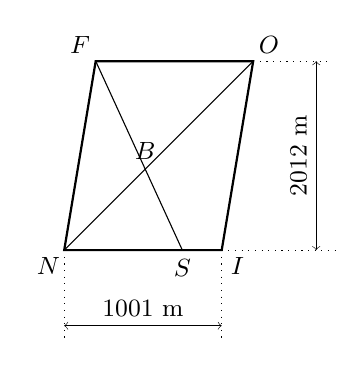
\begin{tikzpicture}[scale=0.8,font=\small]
\usetikzlibrary{calc}

\begin{scope}
%\clip (-2.1,-2.1) rectangle (2.5,2.1);
\coordinate (a) at (0,0);
\coordinate (b) at (2.5,0);
\coordinate (c) at (3,3);
\coordinate (d) at (0.5,3);

\draw[thick] (a) node[shift={(-0.2,-0.2)}] {$N$} -- (b) node[shift={(0.2,-0.2)}] {$I$} -- (c) node[shift={(0.2,0.2)}] {$O$} -- (d) node[shift={(-0.2,0.2)}] {$F$} -- cycle;

\draw[very thin, <->] (0,-1.2) coordinate (n1) -- node[above] {1001 m} (2.5,-1.2) coordinate (i1);
\draw[very thin, <->] (4,0) coordinate (i2) -- node[sloped,above] {2012 m} (4,3) coordinate (o2);

\draw[dotted] (c) -- ($(c)!1.2!(o2)$);
\draw[dotted] (b) -- ($(b)!1.2!(i2)$);
\draw[dotted] (a) -- ($(a)!1.2!(n1)$);
\draw[dotted] (b) -- ($(b)!1.2!(i1)$);

\draw (d) -- ($(a)!0.75!(b)$) coordinate (s) node[below] {$S$};
\draw (a) -- (c);
\coordinate (r) at (intersection of d--s and a--c);
\node[above] at (r) {$B$};

\end{scope}


\end{tikzpicture}

%	\caption{Esercizio~\ref{ese:7.109}}\label{fig:ese7.109}
%\end{figure}

\begin{esercizio}[Giochi d'Autunno 2011]
\label{ese:7.109}
Nel parallelogramma $ABCD$ il segmento $BD$ è perpendicolare ad $AB$ ed $E$ e $F$ sono i punti medi di $AB$ e $CD$ rispettivamente. Calcolare l'area del quadrilatero $GEHF$, sapendo che $AB=5$~cm e $BD=2$~cm.
\end{esercizio}

%\begin{figure}[!htb]
	\centering% Copyright (c) 2015 Daniele Masini - d.masini.it@gmail.com

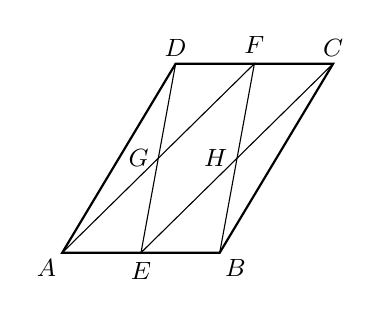
\begin{tikzpicture}[scale=0.8,font=\small]
\usetikzlibrary{calc}

\begin{scope}
\coordinate (a) at (0,0);
\coordinate (b) at (2.5,0);
\coordinate (c) at (4.3,3);
\coordinate (d) at (1.8,3);
\coordinate (e) at ($(a)!0.5!(b)$);
\coordinate (f) at ($(c)!0.5!(d)$);

\draw[thick] (a) node[shift={(-0.2,-0.2)}] {$A$} -- (b) node[shift={(0.2,-0.2)}] {$B$} -- (c) node[shift={(0,0.2)}] {$C$} -- (d) node[shift={(0,0.2)}] {$D$} -- cycle;

\draw (a) -- (f) -- (b);
\draw (c) -- (e) -- (d);

\coordinate (h) at (intersection of e--c and f--b);
\coordinate (g) at (intersection of d--e and a--f);

\node[above] at (f) {$F$};
\node[below] at (e) {$E$};

\node[left] at (g) {$G$};
\node[left] at (h) {$H$};

\end{scope}


\end{tikzpicture}

%	\caption{Esercizio~\ref{ese:7.110}}\label{fig:ese7.110}
%\end{figure}

\begin{esercizio}[Giochi d'Autunno 2010]
\label{ese:7.110}
In un triangolo due angoli misurano rispettivamente $30\grado$ e $105\grado$ ed il lato tra essi compreso è lungo 2~cm. Qual è la misura del perimetro del triangolo? 
\end{esercizio}

\begin{esercizio}[Giochi d'Autunno 2011]
\label{ese:7.111}
In un parallelogramma di area 1~m\textsuperscript{2} le lunghezze di due lati consecutivi sono una il doppio dell'altra. Inoltre uno degli angoli interni misura $60\grado$. Quanto misura la diagonale minore?
\end{esercizio}

\begin{esercizio}[Giochi d'Autunno 2010]
\label{ese:7.112}
In un triangolo equilatero $ABC$ con lato di lunghezza 3~m, prendiamo i punti $D$, $E$ e $F$ sui lati $AC$, $AB$ e $BC$ rispettivamente, in modo che i segmenti $AD$ e $FC$ misurino 1~m e il segmento $DE$ sia perpendicolare ad $AC$. Quanto misura l'area del triangolo $DEF$?
\end{esercizio}

%\begin{figure}[!htb]
	\centering% (c) 2014 Daniele Masini - d.masini.it@gmail.com
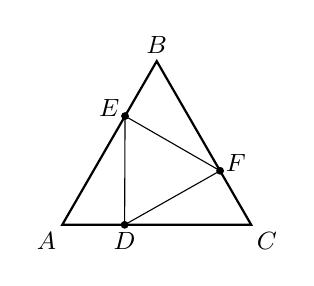
\begin{tikzpicture}[scale=1.2,font=\small]
\usetikzlibrary{calc}

\begin{scope}
\draw[thick] (0,0) coordinate (a) node[shift={(-0.2,-0.2)}] {$A$} -- ++(0:2) coordinate (c) node[shift={(0.2,-0.2)}] {$C$} -- ++(120:2) coordinate (b) node[shift={(0,0.2)}] {$B$} -- cycle;

\coordinate (d) at ($(a)!0.33!(c)$);
\coordinate (f) at ($(c)!0.33!(b)$);
\path (d) let \p1 = (d) in -- ({\x1},{\y1+1}) coordinate (d1);
\coordinate (e) at (intersection of d--d1 and a--b);

\draw (d) -- (e) -- (f) -- cycle;

\draw[fill] (d) circle (1pt) node[shift={(0,-0.2)}] {$D$};
\draw[fill] (e) circle (1pt) node[shift={(-0.2,0.1)}] {$E$};
\draw[fill] (f) circle (1pt) node[shift={(0.2,0.1)}] {$F$};

\end{scope}


\end{tikzpicture}

%	\caption{Esercizio~\ref{ese:7.113}}\label{fig:ese7.113}
%\end{figure}

\begin{esercizio}[Giochi di Archimede 2005]
\label{ese:7.113}
Dato un quadrato $ABCD$ si uniscono i punti medi dei lati aventi un vertice in comune formando un nuovo quadrato $EFGH$. Ripetiamo la stessa operazione per $EFGH$ e otteniamo un nuovo quadrato $A'B'C'D'$. Quanto vale il rapporto tra l'area di $ABCD$ e l'area di $A'B'C'D'$?
\end{esercizio}

\end{multicols}


\subsection{Risposte}

\begingroup
\hypersetup{linkcolor=black}

\paragraph{\ref{ese:7.10}.}
$25/4$~cm.

\paragraph{\ref{ese:7.11}.}
18~cm.

\paragraph{\ref{ese:7.12}.}
$24a^2$.

\paragraph{\ref{ese:7.13}.}
135~cm\textsuperscript{2}.

\paragraph{\ref{ese:7.14}.}
$2p=96a$,\quad $A=93/2a^2$.

\paragraph{\ref{ese:7.15}.}
$AH=20$~cm,\quad $2p=\np{220,1}$~cm.

\paragraph{\ref{ese:7.16}.}
$A=4\sqrt{3}a^2$,\quad $d_1=2\sqrt{3}a$,\quad $d_2=2\sqrt{7}a$.

\paragraph{\ref{ese:7.17}.}
$2p=50a$,\quad $A=150a^2$.

\paragraph{\ref{ese:7.18}.}
$2p=10a(2\sqrt{3}+3)/3$,\quad $A=25a^2/\sqrt{3}$.

\paragraph{\ref{ese:7.19}.}
34~cm,\quad 12~cm.

\paragraph{\ref{ese:7.20}.}
$\frac{3}{4}\sqrt{3}$~m\textsuperscript{2}.

\paragraph{\ref{ese:7.21}.}
$2+\sqrt{6}$~cm\textsuperscript{2}.

\paragraph{\ref{ese:7.22}.}
$2p=28+5(\sqrt{6}+\sqrt{10})$~cm.

\paragraph{\ref{ese:7.23}.}
$4+2/\sqrt{3}$,\quad $4\sqrt{3}+2$.

\paragraph{\ref{ese:7.24}.}
$6+2\sqrt{3}$.

\paragraph{\ref{ese:7.25}.}
$18(1+\sqrt{3})$,\quad $27(4+\sqrt{3})$.

\paragraph{\ref{ese:7.26}.}
$28+8\sqrt{2}$,\quad $80$.

\paragraph{\ref{ese:7.27}.}
$10(1+\sqrt{2})$,\quad $25$.

\paragraph{\ref{ese:7.28}.}
$24(9+\sqrt{3})$,\quad $36+12\sqrt{2}+12\sqrt{3}$.

\paragraph{\ref{ese:7.29}.}
$10+5\sqrt{34}$,\quad $\frac{125}{2}$.

\paragraph{\ref{ese:7.30}.}
$14\sqrt{2}+8\sqrt{6}$,\quad $14\sqrt{3}+24$.

\paragraph{\ref{ese:7.31}.}
$EH=EK=4$~m,\quad $2p=8(\sqrt{3}+1)$~m,\quad $C=8\pi$.

\paragraph{\ref{ese:7.32}.}
a)~$2p=2x(\sqrt{2}+3)$; $A=4x^2$,\quad b)~$2p=2x(4+\sqrt{3})$; $A=2x^2(1+\sqrt{3})$,\quad c)~$2p=2x(2+\sqrt{3})$; $A=2x^2(3+\sqrt{3})$.

\paragraph{\ref{ese:7.33}.}
$\frac{11}{6}a\sqrt{2}+a\sqrt{6}$,\quad $\frac{1}{6}a^2(e+2\sqrt{3})$.

\paragraph{\ref{ese:7.34}.}
$2p=a+3a\sqrt{3}$,\quad $A=\frac{1}{2}a^2\sqrt{3}$.

\paragraph{\ref{ese:7.35}.}
$6a\sqrt{3}+9a$,\quad $\frac{1}{24}(21a^2\sqrt{3}+36a^2)$.

\paragraph{\ref{ese:7.36}.}
$2\sqrt[4]{27}$~m.

\paragraph{\ref{ese:7.37}.}
$4\sqrt{2}$.

\paragraph{\ref{ese:7.38}.}
$18+6\sqrt{10}$.

\paragraph{\ref{ese:7.39}.}
$\np{5,61}$.

\paragraph{\ref{ese:7.40}.}
$\frac{4}{9}\sqrt{3}$.

\paragraph{\ref{ese:7.41}.}
$3/4$.

\paragraph{\ref{ese:7.42}.}
36,\quad 18.

\paragraph{\ref{ese:7.43}.}
12~cm\textsuperscript{2},\quad 12~cm\textsuperscript{2},\quad $172\grado$.

\paragraph{\ref{ese:7.44}.}
$\np{0,665}$,\quad $\np{10,85}$~cm.

\paragraph{\ref{ese:7.45}.}
$\np{300,12}$~mm.

\paragraph{\ref{ese:7.46}.}
36,\quad $\np{0,625}$.

\paragraph{\ref{ese:7.48}.}
42~cm,\quad 108~cm\textsuperscript{2},\quad $\np{7,2}$~cm.

\paragraph{\ref{ese:7.49}.}
$\np{11,25}$~cm\textsuperscript{2},\quad $\np{5,625}$~cm\textsuperscript{2}.

\paragraph{\ref{ese:7.50}.}
$252$~cm\textsuperscript{2}.

\paragraph{\ref{ese:7.51}.}
3~cm,\quad 6~cm\textsuperscript{2},\quad $\np{2,4}$~cm,\quad 5~cm,\quad $\np{3,5}$~cm.

\paragraph{\ref{ese:7.52}.}
100~cm.

\paragraph{\ref{ese:7.53}.}
$\np{33,59}$~cm\textsuperscript{2}.

\paragraph{\ref{ese:7.54}.}
$\np{15,48}$~cm\textsuperscript{2}.

\paragraph{\ref{ese:7.57}.}
$45\grado$,\quad $67,5\grado$.

$\np{42,24}$~cm\textsuperscript{2}.

\paragraph{\ref{ese:7.59}.}
180~cm\textsuperscript{2}.

\paragraph{\ref{ese:7.61}.}
$176\grado13'30''$,\quad $50\grado21'$,\quad $40\grado16'48''$.

\paragraph{\ref{ese:7.62}.}
$\np{1080}$~cm\textsuperscript{2}.

\paragraph{\ref{ese:7.63}.}
384~cm\textsuperscript{2},\quad 80~cm.

\paragraph{\ref{ese:7.64}.}
328~cm,\quad $\np{2880}$~cm\textsuperscript{2},\quad $\np{35,15}$~cm.

\paragraph{\ref{ese:7.65}.}
250~cm\textsuperscript{2}.

\paragraph{\ref{ese:7.66}.}
768~cm\textsuperscript{2},\quad 40~cm.

\paragraph{\ref{ese:7.68}.}
$\np{1500}$~cm\textsuperscript{2},\quad 65~cm.

\paragraph{\ref{ese:7.69}.}
$\np{49,5}$~cm\textsuperscript{2}.

\paragraph{\ref{ese:7.70}.}
200~cm,\quad $\np{2304}$~cm\textsuperscript{2}.

\paragraph{\ref{ese:7.71}.}
84~cm\textsuperscript{2},\quad 252~cm\textsuperscript{2}.

\paragraph{\ref{ese:7.77}.}
40~cm.

\paragraph{\ref{ese:7.79}.}
$54\sqrt{7}$~cm\textsuperscript{2},\quad $84\sqrt{7}$~cm\textsuperscript{2}.

\paragraph{\ref{ese:7.83}.}
224~m,\quad 238~m,\quad $\np{23520}$~m\textsuperscript{2}.

\paragraph{\ref{ese:7.84}.}
6~cm,\quad 10~cm,\quad 8~cm.

\paragraph{\ref{ese:7.85}.}
80~cm,\quad 300~cm\textsuperscript{2}.

\paragraph{\ref{ese:7.87}.}
$14 + 2\sqrt{3}$~cm.

\paragraph{\ref{ese:7.89}.}
$9 + 5\sqrt{3} + 2\sqrt{7}$~cm,\quad $29\sqrt{3}/2$~cm\textsuperscript{2}.

\paragraph{\ref{ese:7.91}.}
$\np{30,2}$,\quad $\np{53,75}$.

\paragraph{\ref{ese:7.92}.}
$\np{22,4}$; $\np{19,5}$.

\paragraph{\ref{ese:7.93}.}
$A=14$.

\paragraph{\ref{ese:7.95}.}
$D(-4;2)$.

\paragraph{\ref{ese:7.99}.}
12~cm.

\endgroup


\cleardoublepage
